\documentclass[a4paper]{article}

%% Language and font encodings
\usepackage[english]{babel}
\usepackage[utf8x]{inputenc}
\usepackage[T1]{fontenc}
\setlength{\parindent}{0em}
\setlength{\parskip}{1em}
\usepackage{framed,lipsum}
\usepackage[dvipsnames]{xcolor}
\usepackage{minted}
\usepackage{subcaption}
\usepackage{pdfpages}


%% Sets page size and margins
% \usepackage[a4paper,top=3cm,bottom=2cm,left=3cm,right=3cm,marginparwidth=1.75cm]{geometry}
\usepackage[a4paper,top=2cm,bottom=2cm,left=1.5cm,right=1.5cm,marginparwidth=1.5cm]{geometry}
\renewcommand{\baselinestretch}{1.2}


%% Useful packages
\usepackage{hyperref}
\hypersetup{
	colorlinks=true,
	linkcolor=blue,
	filecolor=magenta,      
	urlcolor=blue,
}
\usepackage{amsmath}
\usepackage{graphicx}
%\usepackage[colorinlistoftodos]{todonotes}
%\usepackage[colorlinks=true, allcolors=blue]{hyperref}

\begin{document}
	\begin{titlepage}
		\centering
		
		
\includegraphics[width=0.5\textwidth]{udacity_logo.png}\par\vspace{1cm}
		
		{\scshape\LARGE Machine Learning Engineering Nanodegree \par}
		\vspace{1cm}
		
		{\scshape\Large Capstone Project\par}
		\vspace{1.5cm}
		
		{\huge\bfseries San Francisco Bay Area Bike Sharing Data Analysis\par}
		\vspace{1cm}
		
		\includegraphics[width=0.7\textwidth]{BayAreaBikeShare.jpg}\par
		{\small Picture taken in 2014 on \href{http://www.sfbike.org/wp-content/uploads/2014/02/BikeShare_746x488.jpg}{sfbike.org}. \par}\vspace{1cm}
		
		
		{\Large\itshape Zhiwei Lin\par}
		{Santa Clara, CA \\
		\href{zlin1985@outlook.com}{zlin1985@outlook.com}}
		\vfill
		
		% Bottom of the page
		{\large \today\par}		
	\end{titlepage}
	
	\pagebreak
	\tableofcontents
	\pagebreak
	
	\section{Definition}
		\subsection{Project Overview}
		
		This project is to investigate a docked bike-sharing system in San Francisco Bay Area, data collected during 2013-2015 when this system just got launched. Different from bike rentals serving for casual riding over several hours or days, bike sharing focuses more on providing bike service on short trips to solve the "last mile" problem, especially for metropolitan areas. The bike sharing service brings convenience to people in situations where neither driving or walking is efficient.
		
		While dock-less bike sharing systems are expanding over the world with dominant number of share-bikes, dock-based bike sharing systems are still the "mainstream" in the US. Even San Francisco Bay Area, currently the technology innovation center of the world, \href{https://www.recode.net/2017/10/23/16496908/bike-sharing-dockless-limebike-ofo-motivate-citi-bike-spin}{only recently starts seeing the wave of the dock-less bike sharing systems}. It is not foreseeable in the near future whether the dock-based system will be fiercely challenged in the US by the dock-less system due to the nature of less populous cities and the existing somewhat mature business model for the docked system. On the other hand, investigation into the dock-based system is a good attempt if one would like to explore further how to improve a dock-less system. To some extent, the dock-less system can be viewed an extension of a dock-based system with a much larger number of stations.
		
		Bike sharing is becoming more and more popular around the world. To improve the bike-sharing systems to make people's life easier and more enjoyable, it is worth studying this system closely, especially on how people use the share-bikes. There are several datasets available on Kaggle on bike sharing with many kinds of analyses. I will focus on the dataset for \href{https://www.kaggle.com/benhamner/sf-bay-area-bike-share}{SF Bay Area Bike Share} as the data are informative and relatively new.
		
		There is also some helpful discussion in academia reviewed by this paper published in 2016 on the bike sharing:
		\href{https://nacto.org/wp-content/uploads/2016/02/2016_Fishman_Bikeshare-A-Review-of-Recent-Literature.pdf}{Bikeshare: A Review of Recent Literature}.
		
		\subsection{Problem Statement}
		Two major problems will be addressed:
		
		\begin{itemize}
			\item How well can we predict the number of daily trips? During one day, how many sections are there with unique characteristics (e.g. one day divided around noon time)? Will studying individual sections help improve the prediction of daily trip frequency? 
			
			The raw trip data will be transformed with the trip counts in one day and sections within a day. Other relevant data (e.g. the weather) will be merged to form a proper dataset for this problem. Since the outputs (daily trip counts) are continuous values, this is a regression problem. Linear regression algorithm will be applied after necessary feature column transformation.
		
			It is very important to predict the demand of share-bikes at several key sections during a day on each specific date. In particular, high peaks of the share-bike usage need to be handled well in order to ensure an efficient system. The strategy to re-balance docks on all the stations is somewhat critical for the bike-sharing company to operate their business.
			
			\item What are the different behaviors between long-term users ("Subscriber") and short-term users ("Customer")? Can we predict whether the biker is a Subscriber or a Customer based on certain features of a specific trip?
			
			Relevant features from the original data will be selected to form an appropriate dataset and then the corresponding training and testing sets. The outputs are two possible class labels, so this is a classification problem. Classifiers that are well interpretable will be used for the classification for the reason being stated in the following paragraph.
			
			For this problem, the goal is actually not on the result of prediction accuracy, but rather on how to interpret the predicted results when the accuracy / F-score is high enough to show strong correlation between the label and the features. The most important features will be extracted to form guidelines to assist bike-sharing companies to come up with proper promotions to convert short-term customers to long-term subscribers.
			
		\end{itemize}
		
		\subsection{Metrics}
		For the regression problem (predicting the number of bikes in demand), the median absolute error (MAE) will be used as the major metric. It is defined as the median absolute error from the predicted and true values:
		
		\begin{equation}
		MAE = Median(|y_{predicted} - y_{true}|)
		\end{equation}
		
		The MAE can be an intuitive measure on how far the prediction is missing the target. The ratio between the MAE and the average actual daily trip count gives an idea about whether the model is practical for the prediction. For example, if the MAE is only 10\% of the mean daily trip count, it is considered a very good model.		
		
		A secondary metric is the Root Mean Squared Logarithmic Error (RMSLE), suggested by Kaggle for the project \href{(https://www.kaggle.com/c/bike-sharing-demand#evaluation)}{Bike Sharing Demand}. The RMSLE is calculated as 
		\begin{equation}
		RMSLE = \sqrt{\frac{1}{n}\sum_{i=1}^{n}(\log(p_i + 1) - \log(a_i + 1))^2}
		\end{equation}
		
		Where:
		\begin{itemize}
			\item $n$ is the number of entries in the test set
			\item $p_i$ is the predicted count
			\item $a_i$ is the actual count
			\item $\log(x)$ is the natural logarithm
		\end{itemize}
		
		According to this \href{https://www.quora.com/What-is-the-difference-between-an-RMSE-and-RMSLE-logarithmic-error-and-does-a-high-RMSE-imply-low-RMSLE}{link}, RMSLE is usually used when one does not want to penalize huge differences in the predicted and the actual values when both predicted and true values are huge numbers. As the number of trips can be a big number, RMSLE can be a good metric to access the quality of the general prediction. This is a complimentary method to the MAE with the latter measuring the median error. If several samples have big discrepancy in true and prediction values, the MAE is not able to measure that, but the RMSLE can.
		
		For the classification problem (predicting whether the user is a non-subscriber), the F0.5 score will be used as the major metric. This metric gives more focus on the precision so that the result reflects on the behavioral pattern of the non-subscribers with less interference from the subscribers. The formula to calculate F0.5 is \href{)https://en.wikipedia.org/wiki/F1_score}{defined} as:
		
		\begin{equation}
			\begin{aligned}
				F_{0.5} &= (1+0.5^2)\frac{Precision * Recall}{\beta^2 * Precision + Recall}\\		
						&= \frac{(1+0.5^2)*True\ 	Positive}{(1+0.5^2)*True\ Positive + 0.5^2*False\ Negative + False\ Positive}
			\end{aligned}
		\end{equation}
				
		The accuracy of the predictions will be used as the secondary metric. The accuracy is calculated as the ratio of the number of correctly predicted data points to the total number of data points in the test set:
		\begin{equation}
		Accuracy = \frac{\sum_{i=1}^{N} (m_i == n_i)}{N}
		\end{equation}
		
		Where:
		\begin{itemize}
			\item $m_i$ is the predicted category of $i^{th}$ row in the test set
			\item $n_i$ is the labeled category of $i^{th}$ row in the test set
			\item $N$ is the number of entries in the test set
		\end{itemize}	
		
		The accuracy is often a good metric for classification problem, as it calculates the percentage of the correct predictions. However, if we deal with an imbalanced dataset with one dominant label and the other label for much fewer samples, the accuracy is not very helpful. This is why the accuracy is used as a secondary metric in this study.

\clearpage
		
	\section{Data Exploration}
		The original raw data come from \href{https://www.kaggle.com/benhamner/sf-bay-area-bike-share}{SF Bay Area Bike Share} from Kaggle. The dataset can be downloaded from \href{(https://www.kaggle.com/benhamner/sf-bay-area-bike-share/downloads/sf-bay-area-bike-share.zip)}{this link}. This dataset is directly related to the problems that are targeted. It includes all "anonymized bike trip data from August 2013 to August 2015" of the San Francisco Bay Area Bike Share program.
		

		\subsection{Data Import}			
			The size of original data is 660MB when downloaded and about 5GB when unzipped. There are four comma-separated values (csv) data files (station, status, trip, weather) and a SQLite database that contain identical information as in the four csv files. The data of station, trip and weather can be directly imported as Pandas' dataframe object with the function pandas.read\_csv. 
			
			However, the status data is too large to be imported: reading it into a dataframe will cause an error. Fortunately the database also have the identical status information. A peek at the data suggests that this data can be highly compressed. Not all the data are important for the analysis. The bike sharing system keeps updating the status of the number of available bikes and docks in each station for every minute even if there is no activity going on. Only those status changes that involves the change of bike or dock counts will be relevant to the share-bike trip study.
			
			Fortunately, an SQL database is available to work with: a query into the database doesn't require to read all the data into memory first. A function named "bike\_status" is defined to extract status data station by station from the database and save only status changes of the bike or dock counts. A new data file "status\_change.csv" is created to store the status change data. The new file has the size of less than 60MB, which can be handled well by Pandas.
			
			Note that the data conversion process takes 10-15 minutes to finish. Once the new data file is generated, the control parameter "sql\_status" should be set to false so that upon re-running the program only read the "status\_change" file rather than going through the time-consuming process again.
			
			The sizes of the four data are:
			\begin{itemize}
				\item station: (70, 7)
				\item status: (2109513, 4)
				\item trip: (669959, 11)
				\item weather: (3665, 24)
			\end{itemize}
			
			This is real-world data. Neither do I expect the data can be used as it is, nor the information in the data is equally important for the specific problems I propose to tackle with. Nevertheless, it is rather important to take a deep look into each data, try to understand the mechanisms behind by exploring different aspects of the data, convert and select certain features to create the proper datasets for the targeted problems. Each data file will be explored thoroughly before generating the datasets.
			
		\subsection{Station Data}
		First of all, the station data have been found to be very clean with no missing values. This is as expected, because the station information must have been validated manually since the start of the bike sharing program and that shouldn't change very dynamically during two years.
			\subsubsection{Mark Stations on Google Map}
			The stations are physically located at certain places, and it will be nice to get a big picture on where they are on the map. A piece of JavaScript code is used to mark stations on Google Map. If the internet is accessible, the station name will be displayed when a mark is clicked.
			\begin{figure}
				\centering
				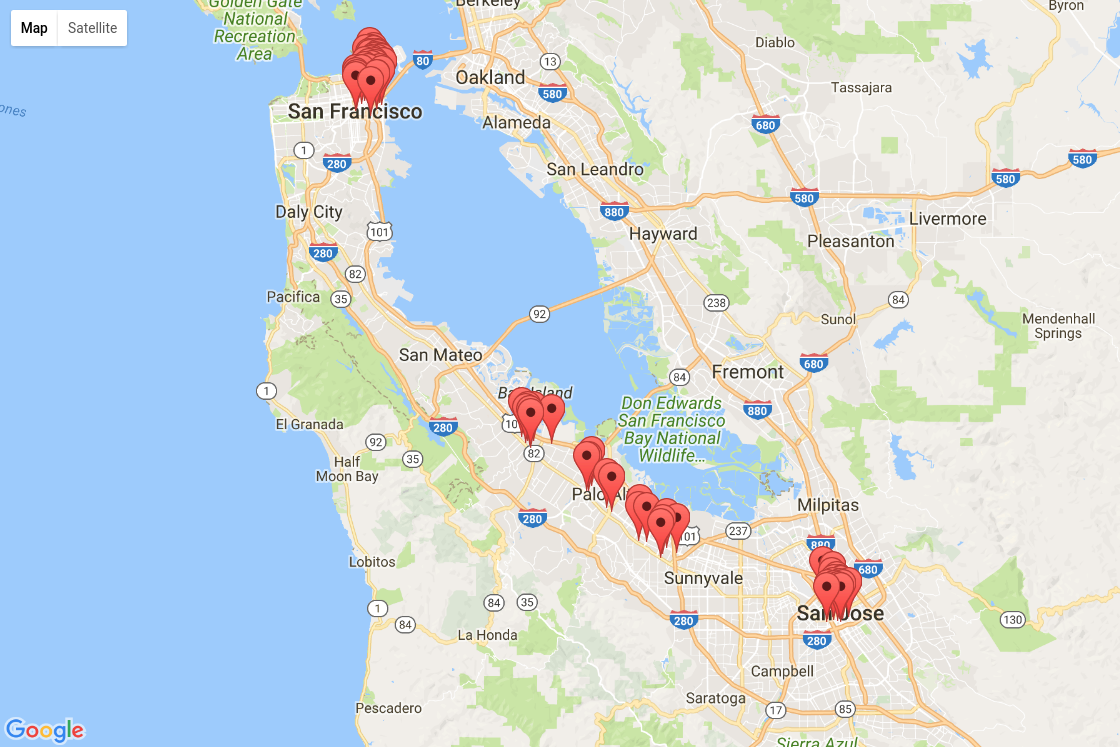
\includegraphics[width=0.8\textwidth]{Station_Map.png}
				\caption{\label{fig:map}The station map is generated from the station.csv data via JavaScript.}
			\end{figure}
			From the map (Figure \ref{fig:map}), we can see that all the stations can be roughly divided into three groups, one in San Francisco, one in San Jose and one between the two cities. In fact, this follows the Caltrain line very well. This makes sense as the bike sharing only solves the last-mile problem, and it must be somehow integrated with other public transportation system to make it run efficiently.
			
			\subsubsection{Heat Map of Docks}
			Different stations don't have the same number of docks available. The design of dock distribution reflects the original expectation of area hotness. A heat map plotted in this section shows the distribution of the docks in the Bay Area.
			\begin{figure}
				\centering
				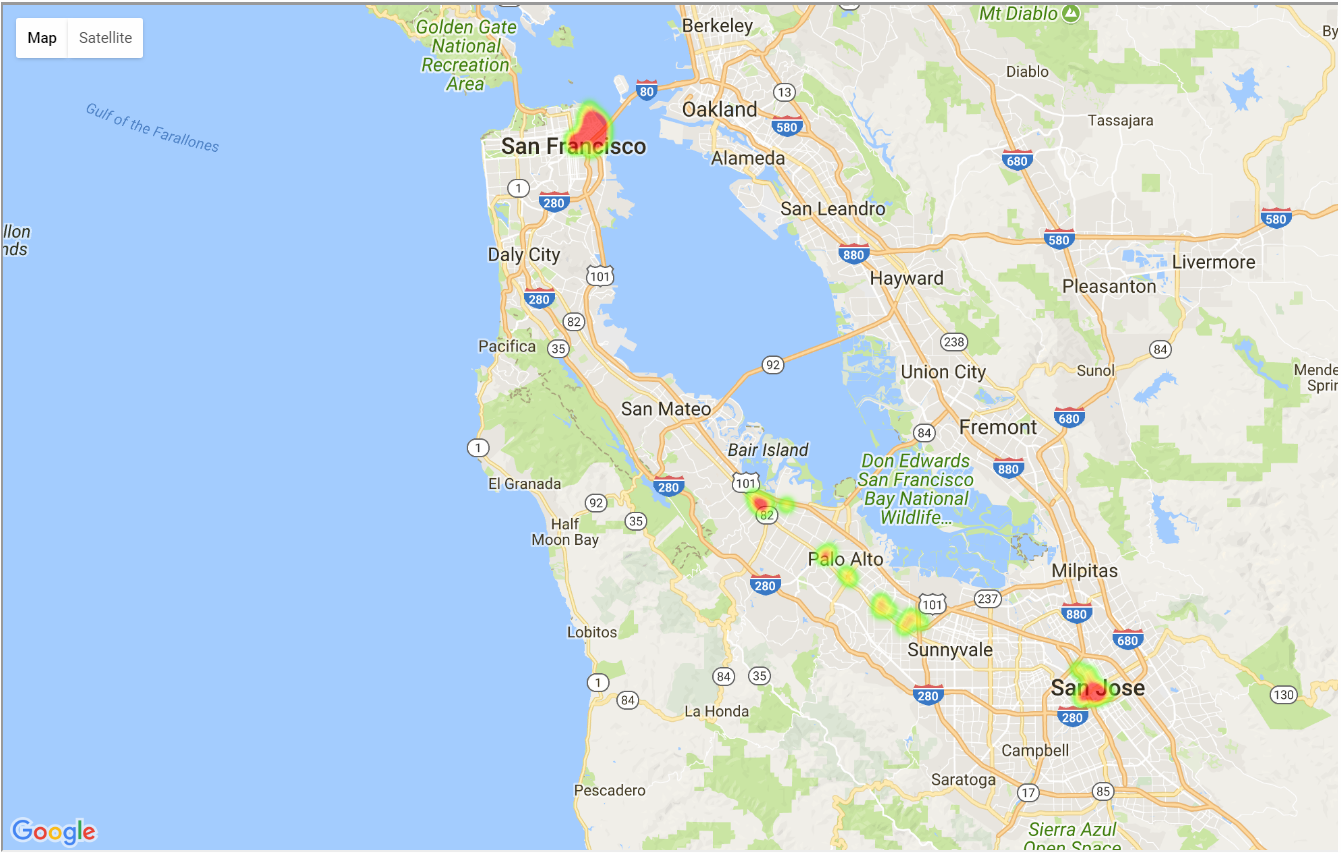
\includegraphics[width=0.8\textwidth]{Docks_HotMap.png}
				\caption{\label{fig:heatmap}The heat map of docks.}
			\end{figure}
			The result (Figure \ref{fig:heatmap}) matches that in the previous section. San Francisco and San Jose are the two hottest spots. The Redwood city is also a hot spot. A mathematical clustering of stations will be explored in the trip data section.
			
			\subsubsection{Station Installation Dates}
			Station installation dates can have significant impact on the prediction of the number of daily trips. As more stations are built, there tends to be more trips. This has something to do the total docks available at a specific date.
			
			As shown in the notebook, most of the stations were built around the same time in August 2013 while the trip data started from the end of August. Nevertheless, there are still a few built later. In populous areas, if many people are using the bike-sharing service, the increase of stations will have quite some effect on the trip counts in that area. The information about the total docks will be used later in the investigation of the regression problem.

		
		\subsection{Trip Data}
			\subsubsection{Cluster Stations}
			As seen on Figure \ref{fig:map}, the stations can be eyed to reside in 3 or 5 groups. This can be confirmed by doing KMeans clustering on the station coordinates (latitude and longitude). Clustering stations by 3 and 5 groups is shown in Figure \ref{fig:cluster}. Note that the graphs shown cannot be directly mapped to the Google Map, because here the west is towards the right and the north is towards the bottom. With the five clusters for example, from north to south, the cluster labels are 0, 3, 1, 4, 2.
			\begin{figure}
				\centering
				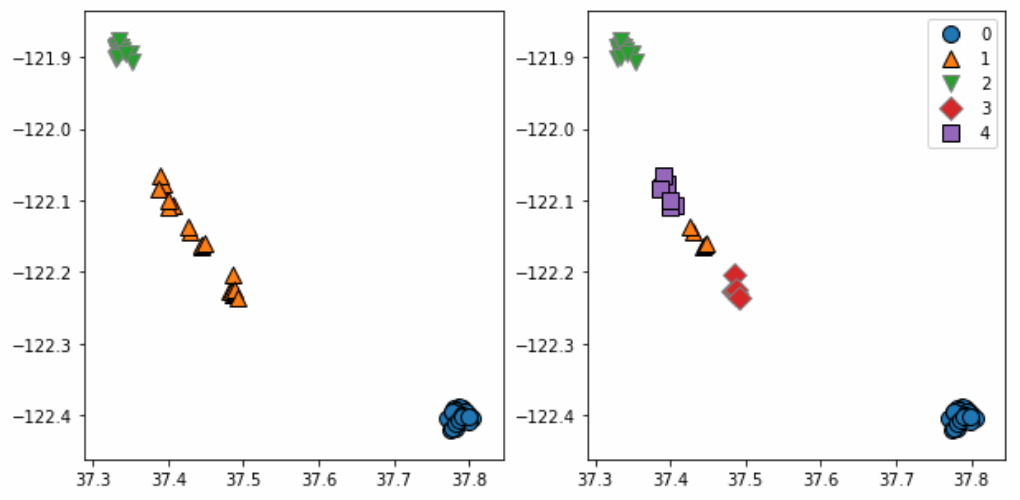
\includegraphics[width=0.8\textwidth]{Clustering.png}
				\caption{\label{fig:cluster}Cluster stations into 3 or 5 groups.}
			\end{figure}
			Clustering the stations is important. Biking has limited distance compared to driving, so most of the bike trips may fall within certain physical regions. Furthermore, regions that are separated distantly from each other may have different weather conditions for the same day which are supposed to have an impact on people's willingness to ride a bike. 
			
			Before delving into the station cluster related exploration, I take a quick look at the trips between stations. It turns out that most of the trips (96.421\%) are between stations. So people use the share-bike mostly to make one-way trips, not round trips without changing the bike.
			
			Opposite to fact that trips between stations are dominant, the inter-group trips are very rare, which is actually the goal of the clustering. The percentage of trips between station groups is 0.011\% if stations are clustered into three groups and 0.156\% if clustered into five. The farther the distance between the two groups, the less the trips between them. Both ways of clustering are fine; clustering into 3 groups may seem even more attractive. However, since the weather data are divided by five unique zip codes, it is better to adopt the 5-group clustering for more natural integration of the trip and weather data. The five zip codes correspond to: 
			
			\begin{itemize}
				\item \ 94107: San Francisco;
				\item \ 94063: Redwood City;
				\item \ 94301: Palo Alto;
				\item \ 94041: Mountain View;
				\item \ 95113: San Jose.
			\end{itemize}    
			
			The five areas defined in the weather data match the station groups when the stations are clustered into five. This also confirms that rationality of the 5-group clustering. A region dictionary is created to map the clustering label to the zip code; a region name dictionary is created to map the zip code to the region names. Note that the KMeans may give a different label for the same group. The label should be ordered according to the longitude of the station group (say from north to south) and then assigned manually to the correct zip code and the name of the city.
			
			A new column is assigned to the trip data to record the station region that the start station of a specific trip belongs to. As the inter-region trips are rare, it doesn't really matter whether the start or the end station is picked to assign the region. The result will not have significant difference.
			
			The percentage of inter-region trips is investigated for different starting regions. As expected, there are almost no inter-region trips from San Francisco and San Jose as they are at the two ends of the map. More inter-region trips (up to 7.09\%) are observed for the rest three regions as they are closer to each other in location. 
			
			The inter-group trips are not negligible for some regions, especially for the three stations that are geographically close to each other. This is another feature to separate different trips. A new column is created to indicate whether a trip is inter-group or not. 
			
			Interestingly, subscribers and non-subscribers contribute to similar number of inter-region trips. Nevertheless, labeling an inter-group trip can still be useful to find out different patterns for different subscription types when other features are taken into account.
			
			\subsubsection{Hourly Trip Counts for Different Subscription Types}
			There are totally 566746 trips done by the subscribers and only 103213 trips by non-subscribers ("customers"). Why is there such a significant distinction? It is worth exploring the behavior patterns for the two subscription types. One natural way to look at it is the hourly trip counts. As a human, a share-bike user must obey the general rule of the human activity. Every day, a typical human wakes up in the morning and sleeps during the night. In the daytime, a human will go for some activities, for work and for fun. 
			
			\begin{figure}
				\centering
				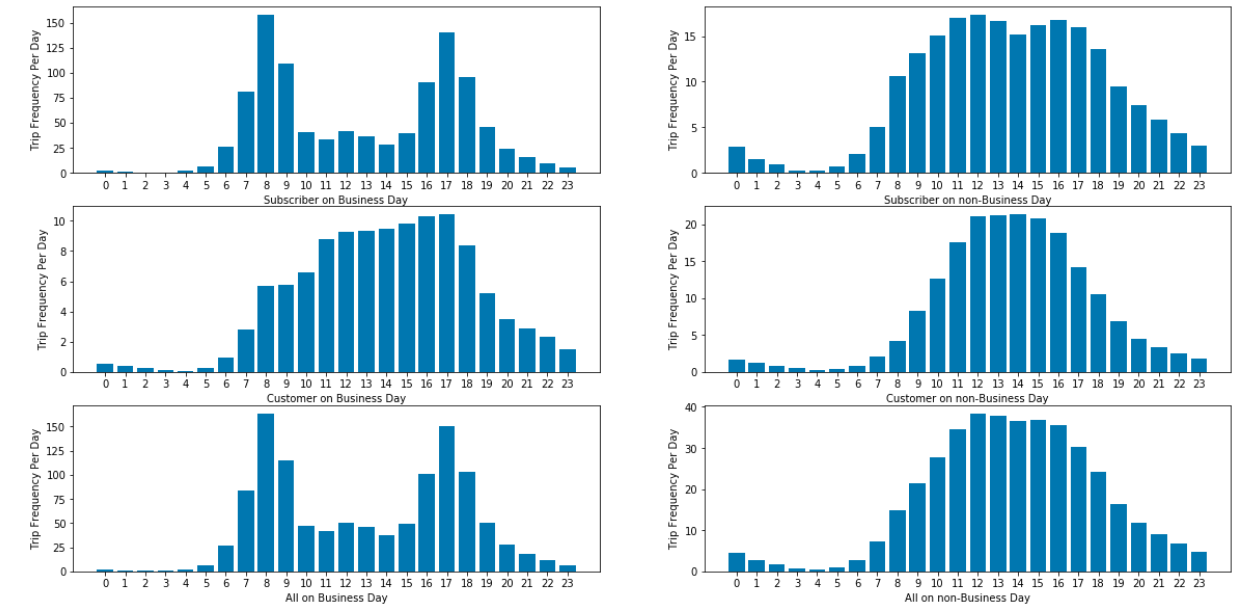
\includegraphics[width=1\textwidth]{HourlyTripsSubs.png}
				\caption{\label{fig:hourly_subs}Hourly trip counts per subscription type.}
			\end{figure}			
			
			As shown in Figure \ref{fig:hourly_subs}, on business days the subscribers' activity has two peaks, one at 8 am and the other at 5 pm: this matches very well with the commuting time for work. On the contrast, non-subscribers don't have such pattern: they are most active during 11 am - 5 pm. It is almost certain to say that on business days, most subscribers use share-bikes as a commuting tool for work, maybe as a complimentary approach to the train. Non-subscribers are more like tourists who are not obliged to work in the Bay Area. 
			
			During non-business days, i.e. weekends and national holidays, there are also two small peaks for subscribers at 12 pm and 16 pm: some people are still working during the weekends and holidays? The pattern for the non-subscribers is very typical for human activity when one is relaxing: people go out and have fun mostly between 12 pm and 3 pm when it is usually the most comfortable daytime in Bay Area.
			
			Pay attention to the number of trip counts. Out of the four patterns discussed above, the trips on business days by subscribers are one order of magnitude larger than the other three. This suggests that the bike sharing makes the most sense in assisting in daily commute to work. Those workers are the major customer group for the bike sharing company. It is also interesting to see the peaking count for non-subscribers during non-business days is not only larger than that during business days, but also larger than that during non-business days done by subscribers. Weekends and holidays are really for non-subscribers / tourists! 
			
			As we can see, there is still a lot room for the bike sharing program to improve for better usage during non-business days and it is so important to reveal the underlying patterns of the non-subscribers. The company can either try to convert them to subscribers, or encourage the tourists to use the share-bikes more. On a different aspect, we can see there are not too many trips per day. Even at peaking hour, there are only about 150 trips, i.e. less than 3 biking activities in one minute, fairly slow.
			
			\subsubsection{Trip Counts for Different Weekdays}
			
			\begin{figure}
				\centering
				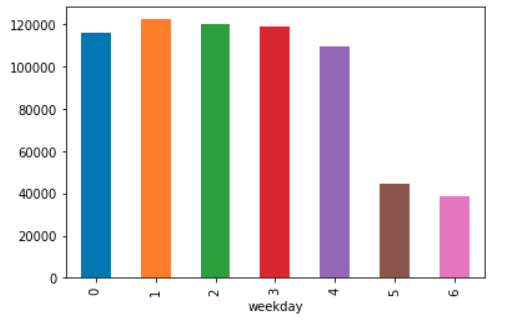
\includegraphics[width=0.5\textwidth]{WeekdayTrips.png}
				\caption{\label{fig:weekday_trips}Trip counts during weekdays.}
			\end{figure}	
			
			Let's see how the trip counts vary on different weekdays in Figure \ref{fig:weekday_trips}. Note that the week starts from Monday and it is labeled 0 instead of 1. Clearly the weekends are the least busy. Monday is a bit slow while Friday is quite slow, comparing to the other weekdays. This matches the common sense when it gets to a typical work cycle during a week in a modern society. People go out and work on weekdays, relax on weekends, start to catch up on Monday and become lazy just before weekends.
			
			\subsubsection{Monthly Trip Counts for Different Subscription Types}
			
			\begin{figure}
				\centering
				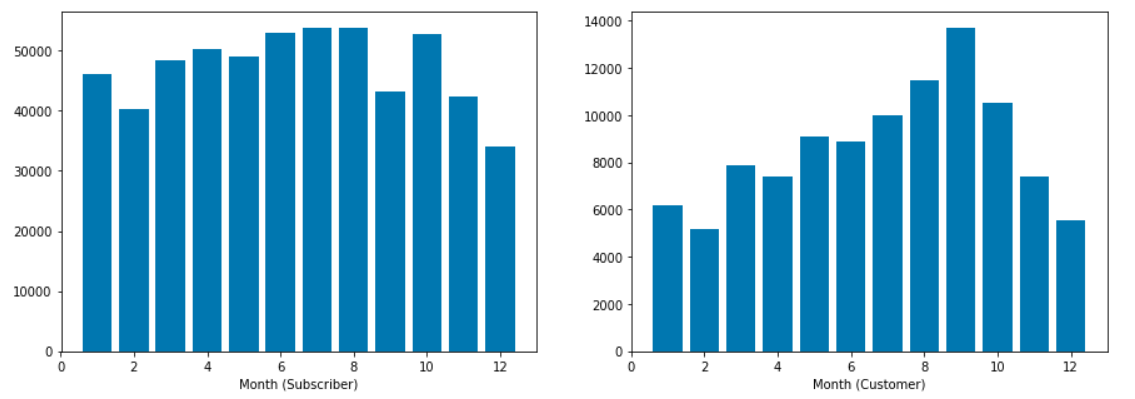
\includegraphics[width=0.8\textwidth]{MonthlyTripsSubs.png}
				\caption{\label{fig:monthly_trips}Monthly trip counts per subscription type.}
			\end{figure}	
			
			There is no significant variation on the number of monthly trips for subscribers except the holiday season (November and December). Interestingly, February and September also observe a significantly lower count. In September, schools for kids begin. Not yet getting used to it, parents may tend to drive cars more often to drop off the kids and then go to work. In February, maybe the drop is caused by the beginning of the lunar year when many Asians are inclined to take days off to enjoy the family get-together? 
			
			For non-subscribers we observe a clear trend of increase from the beginning of the year peaking at September and then decrease: this suggests that the fall is generally a good time to bike in Bay Area for fun and September is the best season for tourists to visit Bay Area. Surprisingly, not many trips for non-subscribers happen during the holiday season when there are supposed to be more tourists. The holiday season in Bay Area is also the raining season: maybe this can explain it.
			
			\subsubsection{Hourly Trip Counts for Station Groups}
			
			\begin{figure}
				\centering
				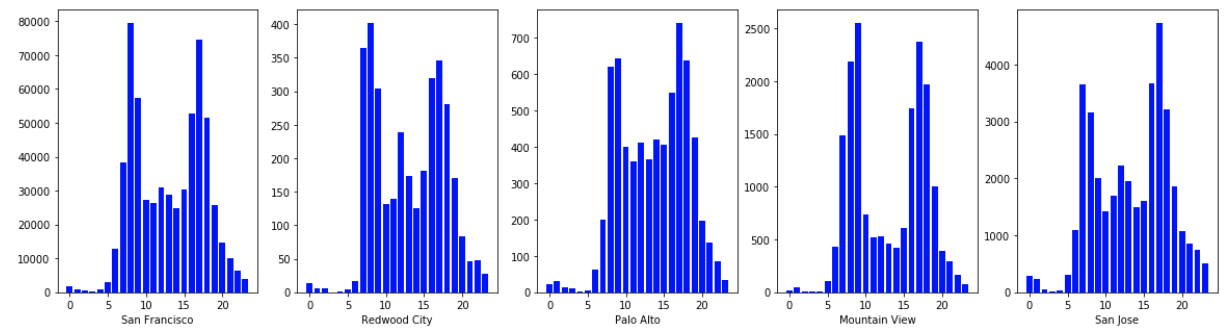
\includegraphics[width=1\textwidth]{HourlyTripsLocation.png}
				\caption{\label{fig:hourly_cities}Hourly trip counts in different cities.}
			\end{figure}	
			
			Now we know how groups of people behave differently across different durations. It is also worth studying how the bike sharing program is doing in each station group or each city. See Figure \ref{fig:hourly_cities}. 
			
			The number of trips in San Francisco is much larger than the other regions. Even the city ranking the second only has a fraction number of trips of it. This is going to skew the data analysis for trips in cities other than San Francisco, so it is necessary to divide the trips into different groups and treat them separately when we try to predict the trip count. 
			
			In the program operation point of view, it makes more sense to predict trip counts per city rather than in all. In case of re-balancing the station with bikes, it is more economic and practical within cities. The reflection on the number of trip counts on each city also helps the company to redesign their current system so that resources can be allocated more efficiently towards cities where most bike trips occur.
			
			The trip frequency pattern varies among cities, but they share a similar feature, that is the two peaks for the work commuting. Mountain View has the most skewed distribution with dominant trips in the two peaks. The relative frequency of people coming out for lunch must be much less than other areas. Is it because of the tech giants like Google in that area? These companies typically offer good lunch for their employees.
				
			\subsubsection{Trip Durations}
			
			\begin{figure}
				\centering
				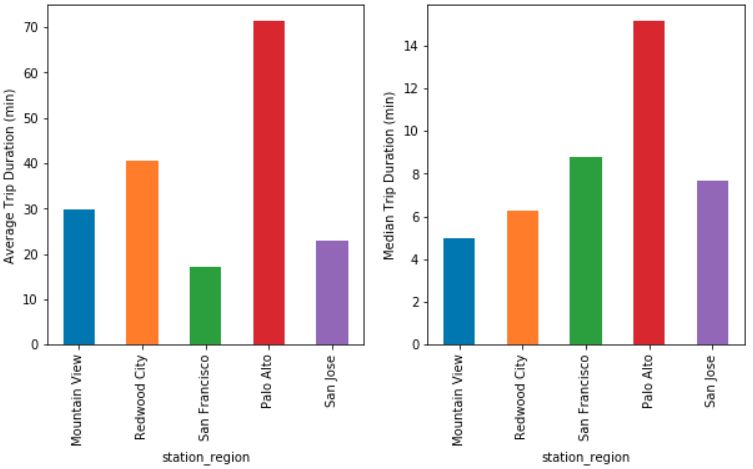
\includegraphics[width=0.8\textwidth]{BikeDuration.png}
				\caption{\label{fig:bike_duration}Average trip duration in different cities.}
			\end{figure}	
			
			Figure \ref{fig:bike_duration} shows the average and median trip duration in different cities. Being the busiest city for bike sharing, San Francisco observes the shortest average trip duration, while not doing bad for median duration. This suggests that most trips in San Francisco are "regular" work trips. Tourists may tend to use the bike longer for touring around. In both criteria, Palo Alto ranks the top: either tourists or students must contribute to it due to the Stanford University in this area. Mountain View and Redwood city must have some very long trips to account for the big ranking drop in median metric compared with the mean metric.
			
			All trips can be divided into 10 groups with minute division points at:
			['4.0', '5.2', '6.3', '7.4', '8.6', '9.9', '11.6', '13.9', '19.2']. Note the last group starts at less than 20 minutes. This means that the almost all trips are less than 20 minutes. More than half of the trips are less than 10 minutes. So most people don't use share-bikes for long trips, which separates well with the bike rental service.
			
			The average trip duration for a subscriber is 9.8 minutes. The average trip duration for a non-subscriber is 65.9 minutes. A non-subscriber tends to have a much longer trip than a subscriber. This is reasonable as most subscribers probably use share-bikes for work commuting while non-subscribers use it for leisure purposes.
			
			\subsubsection{Bike Usage}
			
			\begin{figure}
				\centering
				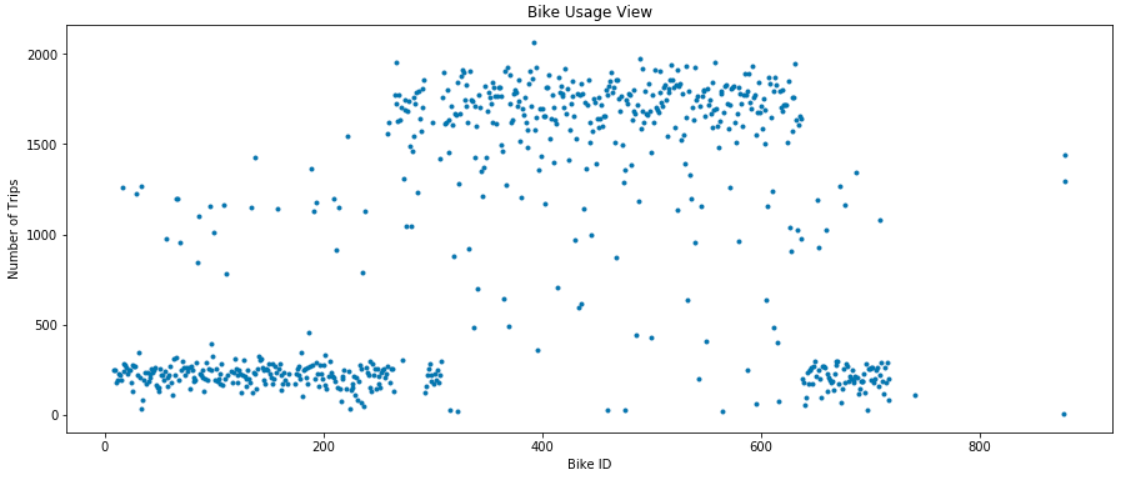
\includegraphics[width=1\textwidth]{BikeUsage.png}
				\caption{\label{fig:bike_usage}Number of trips per bike.}
			\end{figure}	

			If many people are using the bike-sharing service, how long does each bike last? Figure \ref{fig:bike_usage} shows an interesting feature. No matter which bike it is, the number of trips generally does not exceed 2000. At the same time, there are quite some bikes with an average usage of around 250. Does this suggest that the life time of a bike is designed to be up to 2000 before it gets removed out of the bike-sharing system? This is a good guess, but it might not be true. If this is the case, we should expect several levels of bike usage in very busy cities, e.g. San Francisco as a lot of old bikes will be replaced batch by batch with the new bikes. We don't see different levels in the graph.  
			
			\begin{figure}
				\centering
				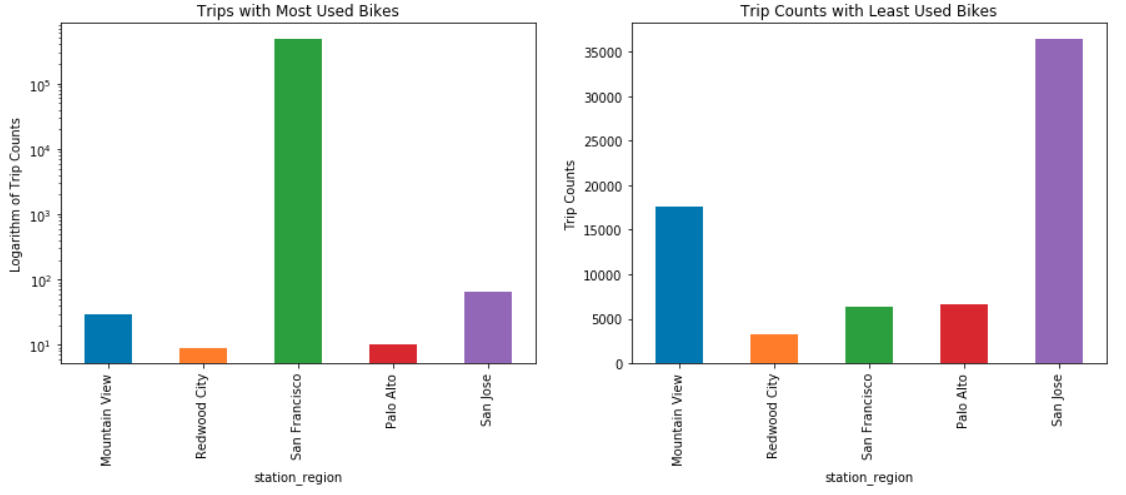
\includegraphics[width=1\textwidth]{BikeUsageRegions.png}
				\caption{\label{fig:bike_usage_region}Where are the most and least used bikes located?}
			\end{figure}				
			
			To explore this further, Figure \ref{fig:bike_usage_region} gives a view on the distribution of the most (> 1500 uses) and the least (< 500 uses) used bikes among different cities. Not surprisingly, the most used bikes are mostly located in San Francisco: note that this is already displayed in log scale. San Jose owns the most least-used bikes. Considering the relatively large dock counts in San Jose compared with the other cities other than San Francisco, it is likely that bikes are just not used very often in cities outside San Francisco. Below I list the trip counts per dock per region in five cities with the least used bikes:

			\begin{itemize}
				\item \ San Francisco: 9.4
				\item \ Redwood City: 28.8
				\item \ Palo Alto: 87.6
				\item \ Mountain View: 150.0
				\item \ San Jose: 137.8
			\end{itemize}    
			
			San Francisco rarely has relatively new bikes. This sort of answers the previous question regarding the lifetime of a bike. Most likely very few bikes have been replaced since the launch date of the bike sharing program. The lifetime of a share-bike may go well beyond 2000 usages. 
			
			The two graphs also demonstrate an interesting point: bikes belonging to one region seem to get used similarly frequently. In San Francisco, it is about 1800, otherwise about 250. This must be intriguing to social scientists as it reveals a pattern of humans as a whole in a society.

			\subsubsection{Local Zip Codes}
			
			\begin{figure}
				\centering
				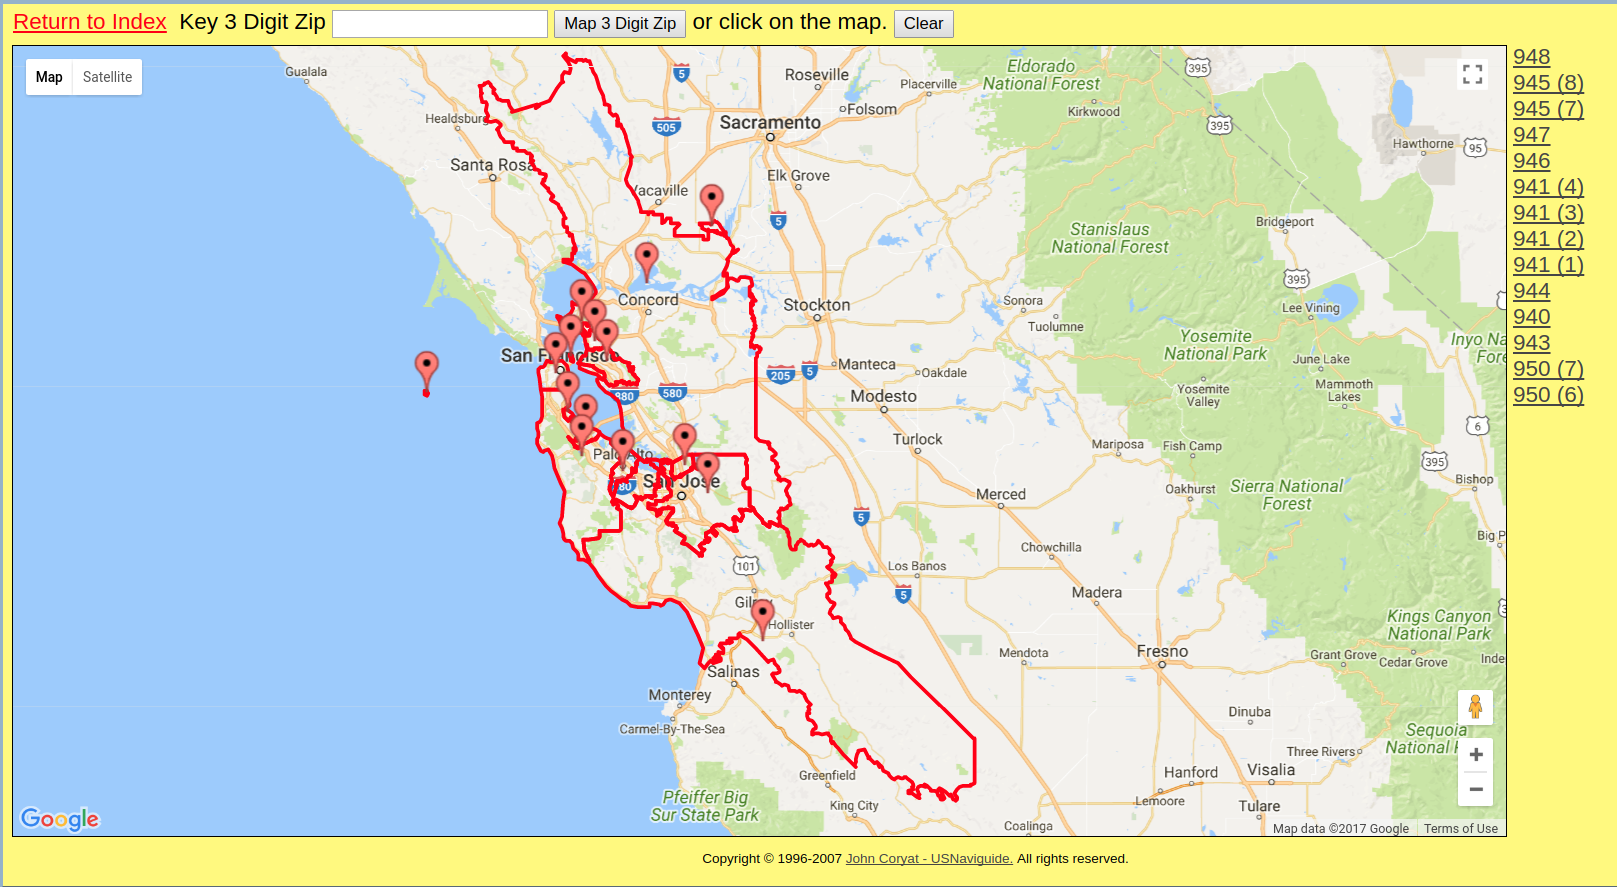
\includegraphics[width=1\textwidth]{Zipcode_Map.png}
				\caption{\label{fig:zipcode}Three-digit zipcode areas.}
			\end{figure}	
			
			As explored earlier, the majority of subscribers can be work commuter while the non-subscribers can mostly be tourists. An important factor to distinguish the two groups is the place they are living: this information can be extracted out from the user's zip code.
			
			The sectional areas with 3-digit zip codes that covers the whole Bay Area are demonstrated in Figure \ref{fig:zipcode}, a screenshot from \href{http://maps.huge.info/zip3.htm}{an online source}. I manually write all the applicable zip codes into a Python list, then create a column for the trip data to indicate if a user has a local zipcode or not. I find that: 89.10\% of the subscribers and 29.28\% of the non-subscribers are local people. This confirms the hypothesis made earlier that most subscribers are local residents, while most of the non-subscribers are tourists.

			\subsubsection{Trip Trend over Time}
			
			\begin{figure}
				\centering
				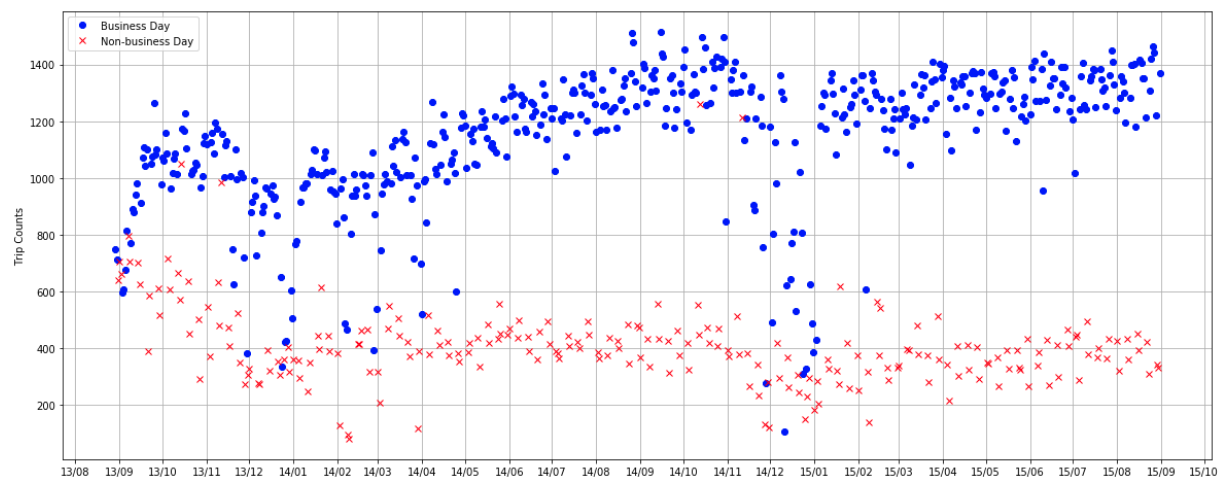
\includegraphics[width=1\textwidth]{TripTrend.png}
				\caption{\label{fig:trend}Trip counts over time.}
			\end{figure}	
			
			Plotting the daily trip counts with the date gives the Figure \ref{fig:trend}. Trip counts separates very well on business days and non-business days. Here are some interesting findings:
			
			For subscribers:
			
			\begin{itemize}
				\item \ There is a sharp rise from 2013/09 to 2013/10 in the trip counts for subscribers, when the program just got launched. We can interpret this as the increasing number of subscribers during this month. Each trip will be labeled whether it is before October 2013 or not as the pattern will clearly be different.
				\item \ A general rise of trip counts since the beginning of 2014 is seen. This could be due to two reasons: 1) people are more aware of this program and start believing that it will bring benefits (maybe because of the marketing) and 2) more stations are built.
				\item \ A clear drop of trip counts are observed in December due to the holiday season.
				\item \ There are some drop during 2014/02 to 2014/05. This could be due to the station construction / modification which happens in 2014/01, 2014/02 and 2014/04.
				\item \ The trip counts in 2015 are very stable. The business becomes mature after 1.5 year's development.
			\end{itemize}   
			
			For subscribers: 			
			
			\begin{itemize}
				\item \ The maximum trip counts are observed in 2013 when the program just got launched. It keeps decreasing until the end of 2013 and gets stable afterwards. Some non-subscribers may turn into subscribers; some may just lose the interest in bike-sharing.
				\item \ There are clearly four outliers in non-business day trips in October and November. An investigation into this finds that these four days are Columbus Day and Veterans Day. This is somewhat shocking to find so many companies in the Bay Area don't have these two holidays off considering they are federal holiday!! These two holidays are labeled as business days with this finding.
			\end{itemize}	

			
		\subsection{Status Data}
			\subsubsection{Total Docks}
			The status data are collected at each station. It has fewer columns than other data: station id, available bikes, available docks and the status time. The raw status data are recorded every minute no matter whether the status changes or not. The data have been preprocessed so that only status changes have been saved. First, I will check if the data is self-consistent.
				\subparagraph{More Docks.}
				If everything is normal, the available bikes and docks should sum up to be the total number of dock counts. 
				
				Two stations (station id 22 and 36) are found to have the total number of docks larger than the originally designed dock counts. Exploring the very beginning and the very end of the two stations helps us to get an idea about the real total dock counts for that station and whether the total docks change during the two years. The total docks in station 22 have been 27 instead of the recorded 25 in the beginning and the end; an update needs to be made for the station data. On the contrary, station 36 has 19 docks, matching the designed dock count. The system may be malfunctioning in station 39 occasionally (188 times) when the total bikes and docks available sums up to 20 or 21, larger than 19. This may also happen due to the relatively coarse temporal step for the status recording.
				
				\subparagraph{Less Docks.}
				
				\begin{figure}
					\centering
					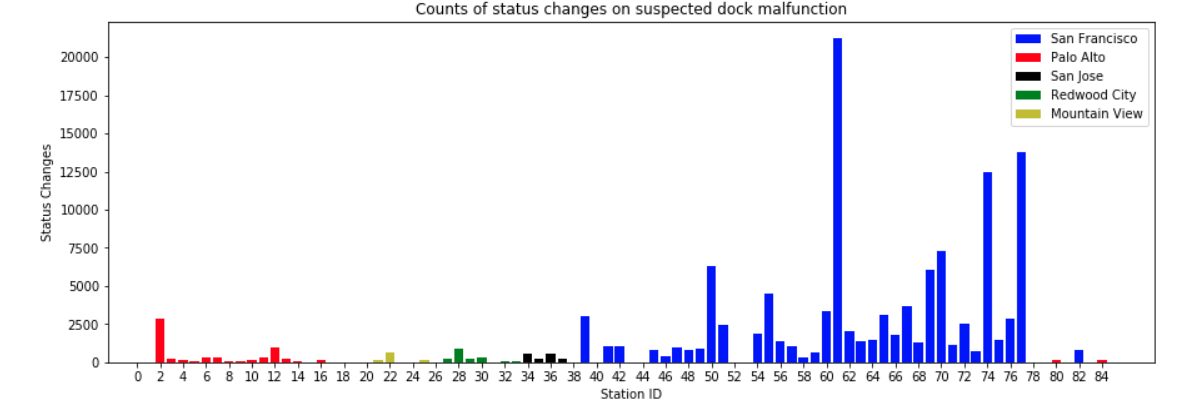
\includegraphics[width=1\textwidth]{LessDocks.png}
					\caption{\label{fig:malfunction}Suspected dock malfunctioning on each station.}
				\end{figure}						
				
				Less dock counts than the total count on paper may imply different issues. As mentioned earlier, the discrepancy of the real dock count recorded by the system and the total count on paper could be ascribed by two reasons: 1) docks malfunctioning, 2) the temporal step in recording the status. For the former, electronic issues or physical damage may be the major causes. I notice this \href{https://www.theguardian.com/us-news/2017/aug/21/bike-sharing-scheme-san-francisco-gentrification-vandalism}{press report} on the vandalism, which could contribute to situation of less docks. The count of suspected dock malfunctioning event is plotted with respect to each station in \ref{fig:malfunction}.
				
				\begin{figure}
					\centering
					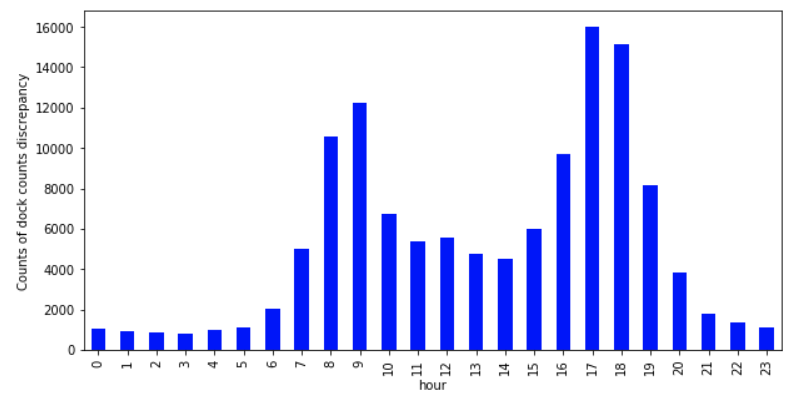
\includegraphics[width=0.8\textwidth]{LessDocksCount.png}
					\caption{\label{fig:less_docks}Dock malfunctioning counts per hour.}
				\end{figure}			
				
				This is actually quite astonishing to see how often the malfunctioning happens.	This is counter-intuitive. To explore it further, I plot the discrepancy event counts with respect to hours in Figure \ref{fig:less_docks}. Interestingly, the pattern of the discrepancy events match the trip frequency very well with two peaks around 9 am and 5 pm. This does not give much information though. If a dock gets damaged and haven't got repaired for an extended period of time, the pattern will resemble the trip pattern. 		
				
				\subparagraph{Total Dock Changes.}				
				
				\begin{figure}
					\centering
					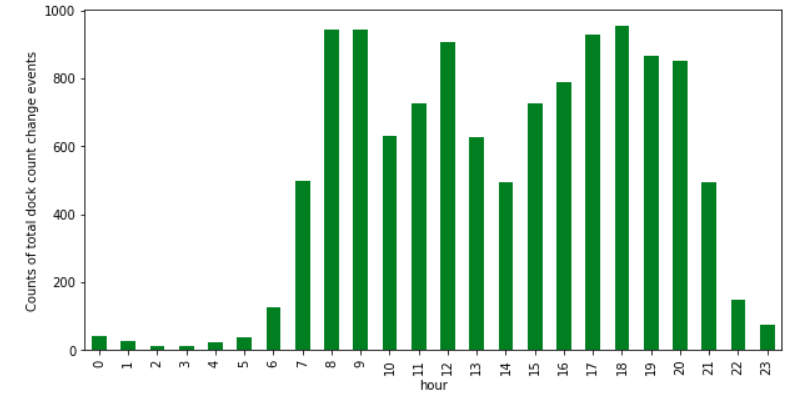
\includegraphics[width=0.8\textwidth]{DockChangeCounts.png}
					\caption{\label{fig:less_docks}Dock count change events.}
				\end{figure}			
				
				To figure it out, I plot the event counts on the total dock count changes (11872 events found) versus hours. This should reflect all the damaging and fixing events. The absolute number sounds to be big, but it only occurs in 0.57\% of the total status changes. Although the malfunctioning happens somewhat often, it is still reasonable for the business operation.			

			\subsubsection{Extra Trips in Status Data}	
			
			\begin{figure}
				\centering
				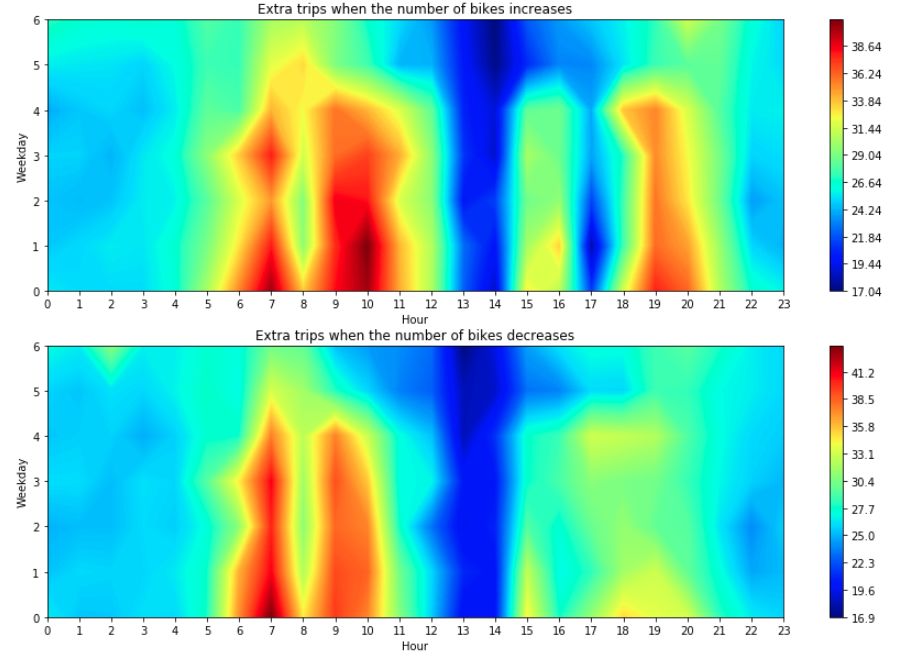
\includegraphics[width=1\textwidth]{WeekdayHour2D.png}
				\caption{\label{fig:extra_trips_2D}Extra trips found in status data plotted in 2D.}
			\end{figure}			
			
			\begin{figure}
				\centering
				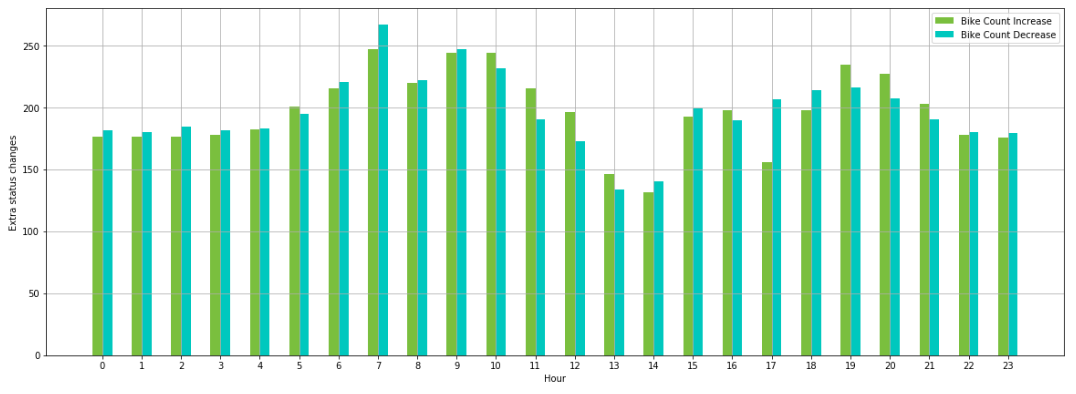
\includegraphics[width=1\textwidth]{ExtraTrips.png}
				\caption{\label{fig:extra_trips_1D}Extra trips found in status data plotted vs. hour.}
			\end{figure}			
			
			The number of status change in status data should match the number of trips in trip data. More specifically, a start of a trip in a specific station should reflect on an decrease of one bike in that station's status. Similarly, an end of a trip in a specific station should reflect on an increase of one bike in that station's status. 
			
			Because the docking system only records the status change once a minute, if several renting and returning events happen during the same minute, the status will only change once. As a rough analysis, I assume that during one minute, a station only sees one type of events, i.e. either renting or returning.
			
			A 2D contour with the averaged number of extra trips per day is plotted vs. the weekday and hour axes (see Figure \ref{fig:extra_trips_2D}). Note that even the blue area are with positive values, which means that all the trip data are reflected in the status data; meanwhile, extra trips always exist. 
			
			The "bike increase" figure shows the end of the extra trips and the "bike decrease" figure shows the start of the extra trips. There is a slight shift from the start to the end in hour during peak hours (e.g. starting at 9 am and ending at 10 am), which suggests the average duration of the extra trips are not very long. 
			
			The activities of the extra trips have four peaks, 7 am, 9-10 am, 3-4 pm and 6-8 pm. Early afternoon is the least active time (1-2 pm). Surprisingly, the extra trips seem to be active from late night to early morning (12 am - 5 am). It is also active during weekends (weekday 5 and 6).
			
			To simplify the analysis, I sum up all weekdays and only look at the hourly change in Figure \ref{fig:extra_trips_1D}. The plotting clearly shows that there are substantial amount of trips going on during night, quite comparable to that during the day.
			
			Some of the extra trips can be explained as the station re-balancing when one station is short of bikes while another station is full of bikes. This can happen a couple of times during a day, but I expect it to happen more often during the daytime on business days.
					
			In fact, there are 73.7\% more trips with bike count increase and decrease in status data, respectively. Why is this? I feel some information missing here. The picture is not clear. This is a bad sign, suggesting that the status data may not be usable in dataset generation. 
			
			The bright side, though, is that the extra trips seem to be real trips as the hourly available bike count increase and decrease roughly match each other, which implies that the trip has a start and an end, not just "ghost" trips.
			
			\subsubsection{When are Stations Empty?}
			
			\begin{figure}
				\centering
				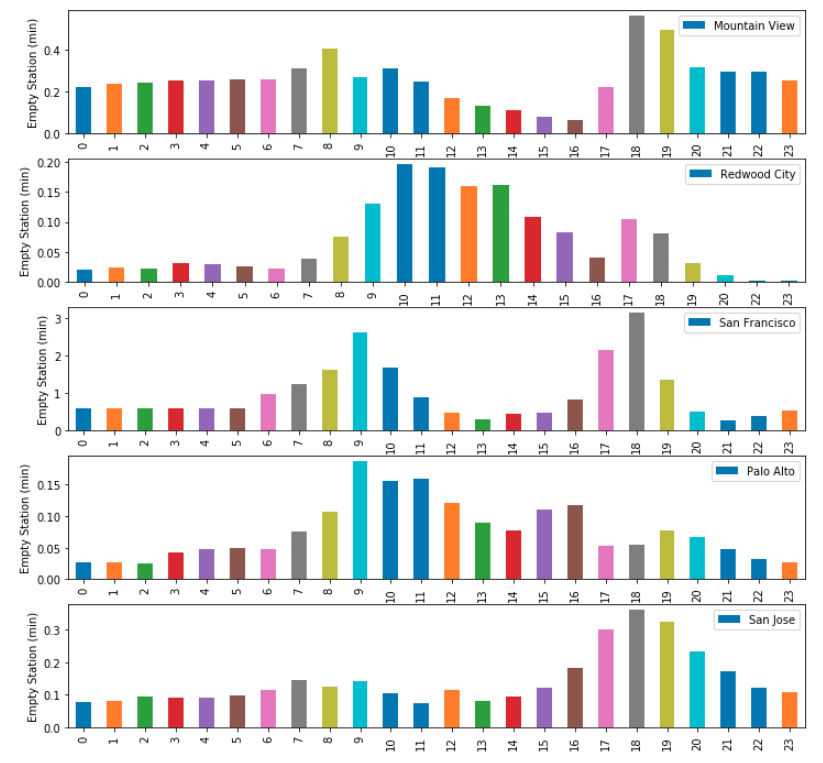
\includegraphics[width=0.7\textwidth]{EmptyStationBDay.png}
				\caption{\label{fig:empty_station_bday}Hourly distribution of events when the station gets empty on business days.}
			\end{figure}			

			\begin{figure}
				\centering
				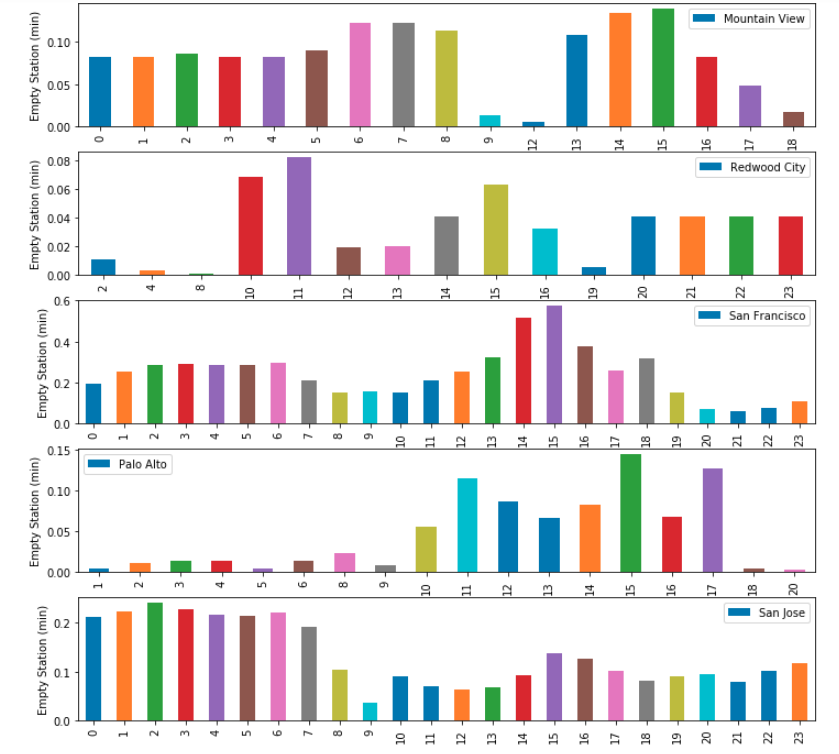
\includegraphics[width=0.7\textwidth]{EmptyStationNonBDay.png}
				\caption{\label{fig:empty_station_nonbday}Hourly distribution of events when the station gets empty on non-business days.}
			\end{figure}			
			
			When do stations run out of share-bikes? This is probably one of the most important questions that a bike-sharing program operator should answer. Not like dock-less bike sharing systems, dock-based system has fixed amount of docks in a station. However, not each station is equally popular. Furthermore, even the same popular station may face different situations at different periods. For example, if one station is surrounded by large companies, one will expect it becomes a hot destination in the morning when all bikes come: maybe more than wanted. In the late afternoon, more bikes may be demanded so that people can leave for home. The opposite will happen for stations that are near the train station in the Central Business District. 
			
			Figure \ref{fig:empty_station_bday} and Figure \ref{fig:empty_station_nonbday} show the hourly distribution of events that a station becomes empty of bikes. On business days, the pattern found in San Francisco matches the trip patter well with two peaks. Other regions don't follow this pattern though. One can compare it with Figure \ref{fig:hourly_cities}. In San Francisco, the share-bike is in good demand for most of the stations, so bikes come and go to form an equilibrium between stations. This makes the trip pattern similar with the station emptiness pattern: when a peak hits, many bikes will be on the road rather than stay in docks. On the other hand, if in general the bike-sharing service is in a low demand in a city, those stations close to interesting points on the map may become full or empty gradually, depending on the time. Other stations will be just quiet. During peak hours, the "hot" station may still have some bikes left; some stations may slowly run out of bikes during non-peak hours. Statistically, it is then hard to see the emptiness pattern matching the trip pattern. Further investigation into this station by station is possible, but this is out of the scope of this study.
			
			On non-business days, the frequency that a region gets into the empty-station status is less, as expected. Noticeably, some bars are thicker -- this means some hours are missing, i.e. not having empty stations. 
			
			Several other findings that worth mentioning here. First, pay attention to the average duration of emptiness. This is calculated for each station by dividing the sum of all the empty events (one minute each) happening at each hour by the number of business / non-business days and then by the number of stations in that region. This is a good metric to judge how big an impact of the empty station on the bike-sharing business. Take San Francisco as an example, during peak hours, there can be up to 3 min of station emptiness among all the stations in this region. On average, this sounds to be an all-right number as it is only 1/20 of the peak hours. In reality, one must investigate it further on each station to come up with a better picture on how to improve certain stations during peak hours. Other regions are all below 1 min, not to mention the situation during non-business days. Another thing is that we always see empty stations during the night. This must be associated with the extra trips: still a mystery to me.
			
			\subsubsection{When are Stations Full?}
			
			\begin{figure}
				\centering
				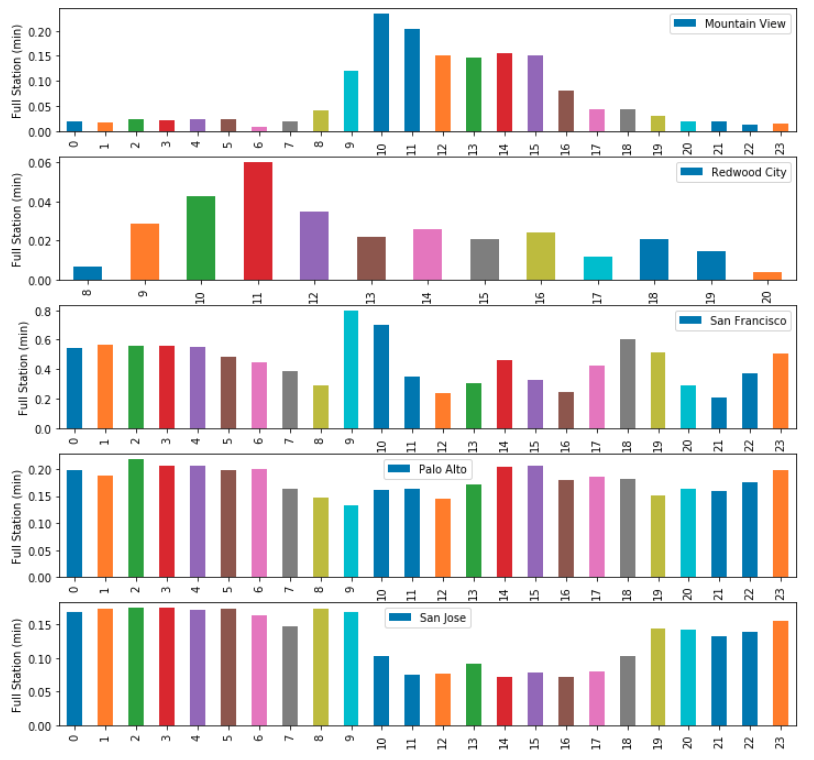
\includegraphics[width=0.7\textwidth]{StationFull.png}
				\caption{\label{fig:full_station}Hourly distribution of events when the station gets no available docks.}
			\end{figure}			
		 
			 There are less events (61.7\%) when the station gets out of available docks than out of available bikes. The event plot also looks interesting (see Figure \ref{fig:full_station}.) The pattern in San Francisco, Palo Alto and San Jose is more or less the same with most events distributed during the night, as common sense suggests. The Redwood City has a very distinct feature. This city does not have a full station during the night at all (9 pm - 7 am). Mountain View has a similar pattern with the Redwood city with few events of station emptiness during the night. Does this imply that most of the bikes used to re-balance other stations come from these city? More information is needed to come to any concrete conclusion, which apparently cannot be done only with the current dataset.
		
		\subsection{Weather Data}
		Weather is a very important factor for the bike-sharing business. After all, biking is an outdoor activity which naturally depends on the outside environment with weather being an inevitable variable. 
		
		A quick exploration of the weather data reveals its nature of high dimension. There are 24 features columns including features of temperature, dew point, humidity, pressure, visibility, wind speed, precipitation, cloud and the associated date and location information. Despite of the many aspects about the weather, some may give redundant information, such as the maximum and mean temperature. This will be investigated in the third sub-section. Before that, the data need to cleaned a bit.		
		
			\subsubsection{Explore the Precipitation Column}
			The precipitation feature is found to be not in numerical values. Two non-number values are found, "T" and nan. 3.9\% of the weather data are labeled "T" for precipitation, while 0.027\% of the weather data are labeled "nan". Some domain knowledge is required here to understand the data. Quoted from \href{ http://www.nws.noaa.gov/om/csd/info/NOWdata/FAQ.php}{NOAA}:
			
			\begin{leftbar}
				\textbf{Looking at daily data, some dates have an "M" or a "T" in the field. What does this mean?}
				
				"M" stands for "Missing". Data for an element will be missing if the primary sensor for that weather element is inoperable (e.g., has an outage) or malfunctioning (e.g., producing errant data) AND any collocated backup sensor is also inoperable or malfunctioning. "T" stand for "Trace". This is a small amount of precipitation that will wet a raingage but is less than the 0.01 inch measuring limit.
			\end{leftbar}
			
			It is reasonable to assign a small value to 'T', 0.005 inches for example. Then the type of this feature column to be float. Only one entry is found to have "nan" value with some other features to be "nan" as well. This will be dealt with in the next sub-section. 
			
			\subsubsection{Deal with NaN Values in Numeric Columns}
			Except the date and zip code columns, other columns all have nan values. To have the best data integration later with the trip data, it would be nice to fill the NaN values instead of simply deleting them. For weather parameters, the best guess for NaN can be the average value of the adjacent days. One can argue that the weather may abruptly change during these days, but an assumption of some mild change is still better than just deleting the whole row. However, the max\_gust\_speed\_mph needs to be investigated independently as there are too many NaN values.
			
			All the selected weather columns are applied with the custom designed function to fill the NaN values with the mean of the adjacent six values (three earlier, three later). The function takes into account the situation for consecutive NaNs following a solution from \href{https://stackoverflow.com/questions/2154249/identify-groups-of-continuous-numbers-in-a-list}{StackOverflow}.
			
			A gust is defined as a sudden increase of the wind’s speed that lasts no more than 20 seconds from this \href{http://www.differencebetween.net/science/nature/difference-between-gust-and-wind/}{web page}. Since the gust is not a weather condition that always exists (like temperature), it is reasonable to assume no gust for NaN values. All the NaNs are replaced by zero.
			
			All NaN values are filled except the events column, which is a categorical feature that will be encoded later.
			
			\subsubsection{Find the Correlations between Features}
			The weather data have too many feature columns, some seeming to be correlated on a first glimpse. To fight against the curse of dimensionality, the strongly correlated columns will be filtered out. This is also a good preprocessing step for machine learning algorithms. Below is quoted from \href{https://datascience.stackexchange.com/questions/24452/in-supervised-learning-why-is-it-bad-to-have-correlated-features}{here}:
			
			\begin{enumerate}
				\item For linear models (e.g., linear regression or logistic regression), multicolinearity can yield solutions that are wildly varying and possibly numerically unstable.
				\item Random forests can be good at detecting interactions between different features, but highly correlated features can mask these interactions.
			\end{enumerate}
			
			The Pearson correlation is calculated between feature columns. The threshold of the coefficient of determination is set to be 0.5 so that more than half of the variance can be explanable. It turns out that:
			
			\begin{itemize}
				\item The mean temperature can well represent the max temperature, the min temperature, the max dew point and the mean dew point, but not the min dew point;
				\item The mean humidity can well represent the max humidity and the min humidity;
				\item The mean sea level pressure can well represent the max sea level pressure and the min sea level pressure.
			\end{itemize}	
			
			All dependent features are removed to reduce the dimension of the data. Then the one-hot encoding is applied to the events column to convert it from categorical to numeric.
			
			It is strange to find low correlation between the max wind speed and the max gust speed. In fact, this depends on the region. The correlation between the max wind speed and the max gust speed is: 
			
			\begin{itemize} 
				\item San Francisco : 0.75
				\item Redwood City : 0.39
				\item Palo Alto : 0.07
				\item Mountain View : 0.51
				\item San Jose : 0.90
			\end{itemize}
			
			\begin{figure}
				\centering
				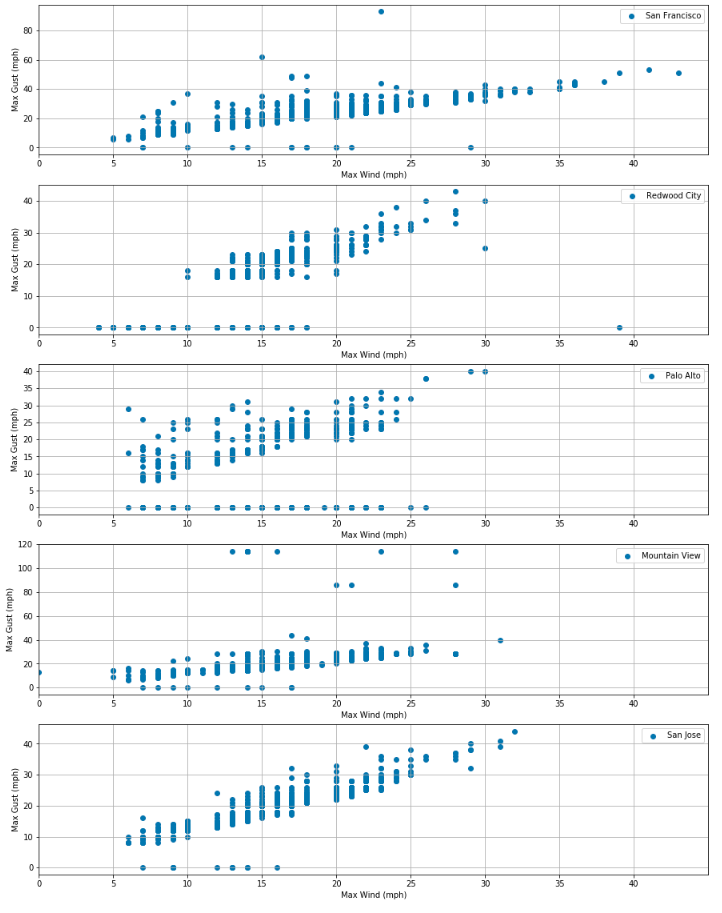
\includegraphics[width=1\textwidth]{WindGust.png}
				\caption{\label{fig:wind_gust}The correlation between the max wind speed and the gust in different stations.}
			\end{figure}			
			
			Interestingly, the correlation is actually high for San Francisco and San Jose while very low for the other three cities. Note that these three cities situate in the deep valley embraced by the mountain to the west and the bay to the east. As shown in Figure \ref{fig:wind_gust}, the max wind speed and the max gust speed are still somewhat linearly correlated but with more variance. Since the overall correlation is not high, I decide to keep both features.
					
			\subsubsection{Monthly Variations}
			
			\begin{figure}
				\centering
				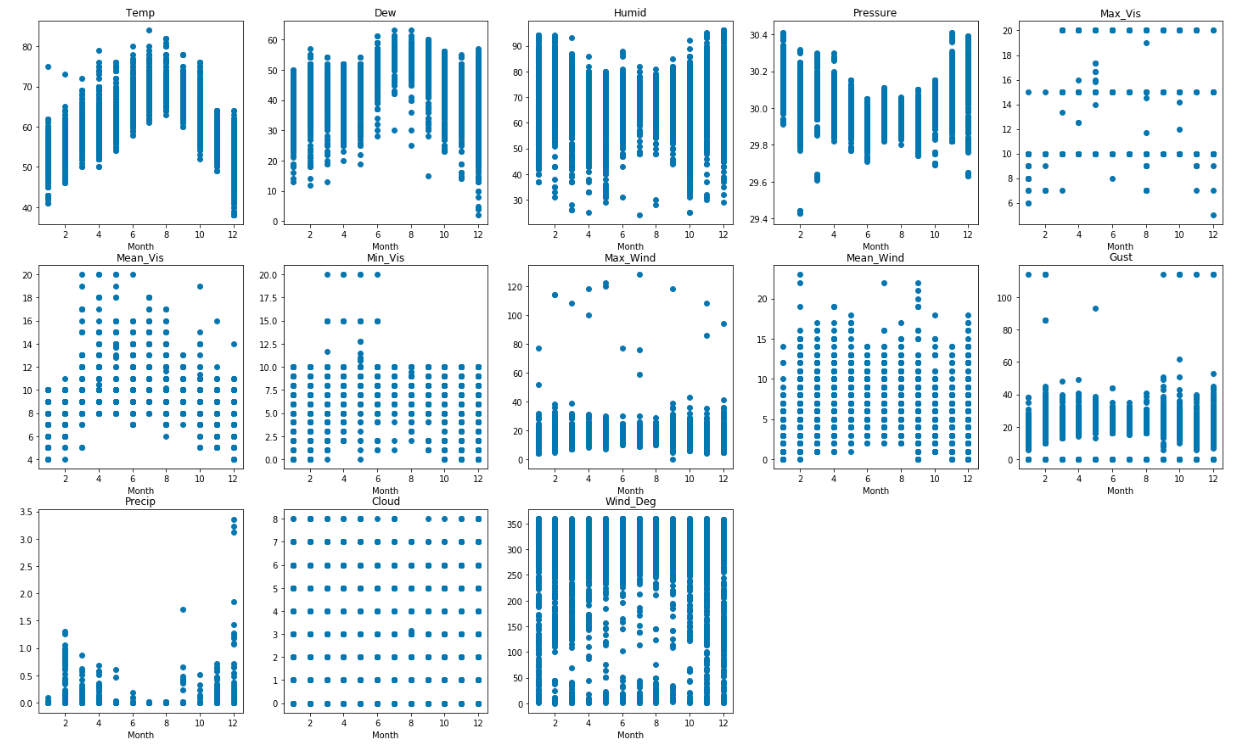
\includegraphics[width=1\textwidth]{WeatherMonthly.png}
				\caption{\label{fig:weather_monthly}Plot all the numeric feature columns versus months.}
			\end{figure}			
			
			Since weather variables usually have seasonal change, I plot all the weather features versus the month in Figure \ref{fig:weather_monthly}. The following weather variables have the most distinct patterns: temperature, dew point, sea level pressure, mean visibility, precipitation, and the wind degree. These can be useful reference for later data analysis. No apparent outliers are observed in these plots.
		
		\subsection{Discussion on the Difficulties and Complications Encountered During the Data Exploration}
		
		The data exploration is no easier than the algorithm implementation below. In fact, this is the most time-consuming part. Besides the feature engineering that required some inspiration, some coding was challenging. Here are some examples:
		
		\begin{itemize}
			\item On the station data, to mark the stations on Google Map, I had to learn JavaScript. 
			
			\item On the trip data, the cluster2cluster function is somewhat complicated to create while the functionality is simply. To extract information from the date was challenging, including the datetime object conversion, business day and holiday assignments. 
			
			\item On the status data, the SQL language was learned to read the data from the database. It was also difficult to disentangle the hidden complex information in the data. I even found extra trips and tried to explain that. Some advanced plotting (2D plots) was tried, too. It was also not easy to admit the fact that the status data is not suitable for dataset generation after a long journey of exploration.
			
			\item On the weather data, quite some domain knowledge was required to clean up the data. 
		\end{itemize}
				
\clearpage
	
	\section{Datasets Generation}
	Now that all the four raw data have been thoroughly explored. We can start building proper datasets to tackle the two problems set earlier. Since the constructed dataset contains the testing set that will be split out later, one must be careful in including feature columns into the dataset, especially for problems that aim in predicting the future rather than just figuring out some patterns. In this study, the regression problem is categorized as the former, while the classification problem is the latter.
	
		\subsection{Regression Problem}
		The goal of tackling the regression problem is to predict the daily trips in the future. Thus, only those features that we know in advance or that can be forecast in the future will be used. Anything that is related to the statistics of the trips during the day is not appropriate as the feature, e.g. the average duration of the trips, the ratio of subscribers over non-subscribers, the frequency of inter-group trips, the number of people that comes from a local zip code, etc. On the contrast, a specific date in the future has the following information known beforehand: the year, month, day, whether it is a business day or before October 2013 (a past time point), which weekday it is, etc. 
		
		However, one needs to be careful when using the year information. Since we are predicting the future, the year may either be irrelevant or can leak information from the testing set to the training set if some data in that year are included in the training set. So I decide not to include the year as a feature for the regression. 
		
		The five regions are found to have different trip patterns in the earlier discussion, so five datasets for regression will be created for different regions. Besides, within one dataset for a region, two sub-datasets with the division at the middle of the day are created for further discussion on the prediction model improvement. 
		
		The label column with the daily trip counts is generated by counting the trips for each date. All relevant feature columns with variables that stay the same for a specific date will be condensed by picking the median value of the day: supposedly these values should be the same for a day and the median value is a robust representation of that value. 
		
		The weather data are now merged with the treated trip data based on the date index. Both data have their date column converted to datetime object earlier so that they can be directly compared. Not all the regions are found to have the same number of days, so care needs to be taken when merging the trip data with the weather data (inner merge).
		
		Lastly, a new column for total dock counts for each day is added to the dataset. The number of total counts is an important parameter for trip count prediction. Now the dataset is ready for the regression problem.
		
		\subsection{Classification Problem}
		The classification problem targets the behavior pattern of the non-subscribers. It is a valid assumption that people's behavior does not change much during a few years, especially for tourists. Therefore, this pattern is not sensitive to time. We don't have to worry about the information leaking from the testing set. 
		
		The shape of the merged data from the trip and weather data is double checked to make sure the merging is correct: the number of rows should match that of the trip data. The date column is removed. A redundant region column is also removed. The classification dataset is completed by one-hot encoding the station region column. In the end, verify that the data don't contain NaN values. The dataset for the classification problem is also ready.		

\clearpage

	\section{Data Analysis}
		\subsection{Regression Problem for Daily Trip Counts Prediction}
		I start realizing more aspects of the problem as this project goes. With the data coming from the real world, the most important question is not to solve a pre-defined problem, but to find the best problem to tackle with. The ultimate goal of the data exploration and analysis should be kept in mind all the time: the focus of the problem may shift as the exploration goes deeper.
			
			\subsubsection{Benchmark Model}
			There are some discussions around this data on Kaggle. The closest analysis to my first set problem is from a notebook named \href{https://www.kaggle.com/currie32/a-model-to-predict-number-of-daily-trips/notebook}{A Model to Predict Number of Daily Trips}. A weighted model from random forest regression, gradient boosting regression and XGBoost is used for the prediction, which can be considered a benchmark model to compare with. The author concludes that:
			
			\begin{leftbar}
				\texttt{My model has a median absolute error of almost 47 trips per day. This should give the company operating this service a good, general estimate of the traffic that will occur each day.}
			\end{leftbar}
			
			Another benchmark result comes from a different bike-sharing dataset: \href{https://www.kaggle.com/c/bike-sharing-demand/}{Bike Sharing Demand}. Also using the Root Mean Squared Logarithmic Error as the metric, the best score on its \href{https://www.kaggle.com/c/bike-sharing-demand/leaderboard}{public leaderboard} is 0.33756. The model is not open to public though.
			
			Both can potentially serve as benchmark results, but note that slightly different problems are targeted by the above-mentioned two solutions. The data used in the first solution is the same as the one in this study, but with different feature engineering. The second solution even uses a different dataset, in spite of the similar target problem.
			
			Neither results can be directly compared. Thus, a naive predictor will be set as the benchmark model instead. The naive predictor will always predict the median value of the label column from training set. This is the best that one can guess without in-depth analysis into the data.
			
			\subsubsection{Predict the Number of Daily Trips for Each Station}
			First, only the daily trips without the sub-divisions are considered. A quick exploration indicates that the gradient boosting regressor is a good model. Applying this algorithm to five regions gives good results compared to the benchmark model. The benchmark model is a naive predictor that always predict the daily trip count as the median trip count of label column in the training set. This is a better benchmark model than that using the averaged value as we expect a large range of trip counts. The median absolute error is used as the metric. The results are listed below:
			
			\begin{itemize}
				\item For San Francisco (median 917 trips daily with 662 docks):
				The median absolute error for the regular prediction is 56.8.
				The median absolute error for the benchmark prediction is 260.0. 
				
				\item For Redwood City (median 4 trips daily with 113 docks):
				The median absolute error for the regular prediction is 2.2.
				The median absolute error for the benchmark prediction is 2.0. 
				
				\item For Palo Alto (median 9 trips daily with 75 docks):
				The median absolute error for the regular prediction is 3.1.
				The median absolute error for the benchmark prediction is 3.0. 
				
				\item For Mountain View (median 26 trips daily with 112 docks):
				The median absolute error for the regular prediction is 3.9.
				The median absolute error for the benchmark prediction is 13.5. 
				
				\item For San Jose (median 55 trips daily with 257 docks):
				The median absolute error for the regular prediction is 9.0.
				The median absolute error for the benchmark prediction is 13.0. 
			\end{itemize}
			
			The prediction of trip count for San Francisco is already pretty good. The error is only 56.8 / 917, which is about 6\%. Before further investigation, I notice the low numbers of daily trips compared to the total docks available. This result is astonishing! Except San Francisco, there are so few trips in a day. The number of trips in San Francisco is higher than the docks, while in other cities not all bikes are used daily! The prediction with the regressor performs even worse than the a random guess for those stations with very small median daily trips, i.e. in Redwood City and Palo Alto. The regressor performs much better than the benchmark for the other three cities.
			
			I had assumed that the bike-sharing is a great business among all the regions. Regions outside San Francisco are expected to be less busy, but I did not anticipate it to be so bad. Take Redwood City as an example. It has 113 docks for the region, but the median number of trips is a single digit. What a waste of resources! The critical problem for these stations is not to improve the re-balancing to more efficiently use the bike-sharing resources, but to set a better strategy to encourage people to use share-bikes in these regions. The strategy can be a better marketing, good promotional plans for trips in these regions, or even a re-design of the system to distribute the docks in a better way, etc. None of these can be solved well by applying machine learning techniques to the current dataset.
			
			Only the San Francisco data are worth further exploration for the daily trip count problem. Below I will focus only on this dataset, neglecting all others. 

			\subsubsection{Improve the Model for San Francisco Trip Data}
			The following describes a detailed process to for model refinement.
			
				\paragraph{Normalize Numeric Feature Columns.}
				First, all the numerical columns are scaled to have values within 0 and 1. The training set and the testing set is then split.				
				
				\paragraph{Select Proper Models by Investigating All Regressors.}
				
				\begin{figure}
					\centering
					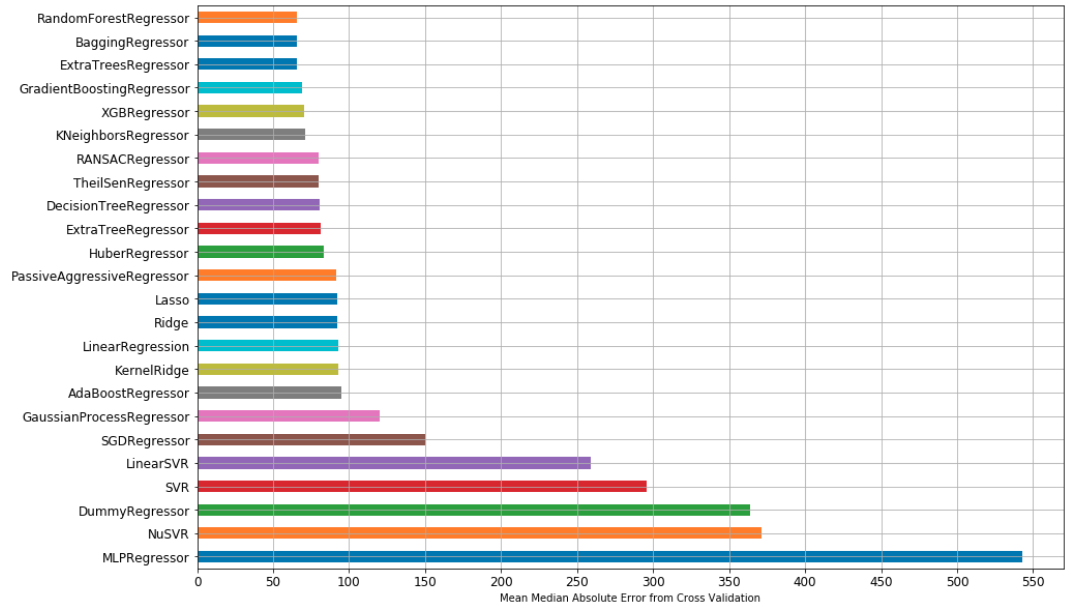
\includegraphics[width=1\textwidth]{Regressors.png}
					\caption{\label{fig:regressors}Scoring for all regressors.}
				\end{figure}	
				
				A scoring function is designed to return the mean scores from the cross validation. The metric is set to the median absolute error. The shuffle split is used to generate 15 cross validation sets: it is well suited for regression analysis.
				
				All applicable regressors from the sklearn packages and the popular xgboost are surveyed to have an overview of performance with their default setting (Figure \ref{fig:regressors}). Note that some regressors have changed their default parameters for different sklearn versions; these warnings are ignored to clean up the results.
				
				The regressors are briefly described as follows (mostly from \href{http://scikit-learn.org/stable/supervised_learning.html#supervised-learning}{sklearn website}):
				\begin{itemize}
					\item Random Forest Regressor: a meta estimator that fits a number of classifying decision trees on various sub-samples of the dataset and use averaging to improve the predictive accuracy and control over-fitting.
					
					\item Bagging Regressor: an ensemble meta-estimator that fits base regressors each on random subsets of the original dataset and then aggregate their individual predictions (either by voting or by averaging) to form a final prediction.
					
					\item Extra Trees Regressor: a meta estimator that fits a number of randomized decision trees (a.k.a. extra-trees) on various sub-samples of the dataset and use averaging to improve the predictive accuracy and control over-fitting.
					
					\item Gradient Boosting Regressor: gradient boosting for regression. GB builds an additive model in a forward stage-wise fashion; it allows for the optimization of arbitrary differentiable loss functions. In each stage a regression tree is fit on the negative gradient of the given loss function.
					
					\item XGB Regressor: XGBoost is an implementation of gradient boosted decision trees designed for speed and performance. XGB Regressor is the regressor version of the XGBoost.					
					
					\item K-Neighbors Regressor: regression based on k-nearest neighbors. The target is predicted by local interpolation of the targets associated of the nearest neighbors in the training set.
					
					\item RANSAC Regressor: RANSAC (RANdom SAmple Consensus) algorithm. RANSAC is an iterative algorithm for the robust estimation of parameters from a subset of inliers from the complete data set. More information can be found in the general documentation of linear models.
					
					\item Theil-Sen Regressor: a robust multivariate regression model. The algorithm calculates least square solutions on subsets with size n\_subsamples of the samples in X. Any value of n\_subsamples between the number of features and samples leads to an estimator with a compromise between robustness and efficiency. In a final step, the spatial median (or L1 median) is calculated of all least square solutions.
					
					\item Decision Tree Regressor: A decision tree regressor.
					
					\item Extra Tree Regressor: an extremely randomized tree regressor. Extra-trees differ from classic decision trees in the way they are built. When looking for the best split to separate the samples of a node into two groups, random splits are drawn for each of the max\_features randomly selected features and the best split among those is chosen. Note that this is different than the Extra Trees Regressor which is an ensemble method.
					
					\item Huber Regressor: a linear regression model that is robust to outliers. The Huber Regressor optimizes the squared loss for the samples where |(y - X'w) / sigma| < epsilon and the absolute loss for the samples where |(y - X'w) / sigma| > epsilon, where w and sigma are parameters to be optimized. 
					
					\item Passive Aggressive Regressor: the passive-aggressive algorithms are a family of algorithms for large-scale learning. They are similar to the Perceptron in that they do not require a learning rate. 
					
					\item Lasso: a linear Model trained with L1 prior as regularizer (aka the Lasso). LASSO is an acronym for Least Absolute Selection and Shrinkage Operator.
					
					\item Ridge: this model solves a regression model where the loss function is the linear least squares function and regularization is given by the L2-norm.
					
					\item Linear Regression: ordinary least squares Linear Regression.
					
					\item Kernel Ridge: this is the kernel ridge regression (KRR). KRR combines ridge regression (linear least squares with L2-norm regularization) with the kernel trick. It thus learns a linear function in the space induced by the respective kernel and the data. 
					
					\item Ada Boost Regressor: a meta-estimator that begins by fitting a regressor on the original dataset and then fits additional copies of the regressor on the same dataset but where the weights of instances are adjusted according to the error of the current prediction. As such, subsequent regressors focus more on difficult cases.
					
					\item Gaussian Process Regressor: Gaussian Processes (GP) are a generic supervised learning method designed to solve regression and probabilistic classification problems. The GaussianProcessRegressor implements Gaussian processes (GP) for regression purposes.
					
					\item SGC Regressor: a linear model fitted by minimizing a regularized empirical loss with SGD. SGD stands for Stochastic Gradient Descent: the gradient of the loss is estimated each sample at a time and the model is updated along the way with a decreasing strength schedule (aka learning rate).
					
					\item Linear SVR: Linear Support Vector Regression.
					
					\item SVR: Epsilon-Support Vector Regression. The default kernel is 'rbf', the radial basis function kernel.
					
					\item Dummy Regressor: a regressor that makes predictions using simple rules. The default strategy is 'mean', which always predicts the mean of the training set.
					
					\item Nu SVR: Nu Support Vector Regression. The implementation is based on libsvm.
					
					\item MLP Regressor: Multi-layer Perceptron regressor. This model optimizes the squared-loss using LBFGS or stochastic gradient descent.
				\end{itemize}
				
				For regressors, the dummy regressor which always predicts the mean value of the training set and the plain linear regression model (LinearRegression, Lasso or Ridge) can be two benchmark models to compare with. Interestingly, some regressors perform worse than the dummy regressor (random guess): NuSVR and MLPRegressor. This doesn't necessarily mean that these two algorithms are not good. It only suggests that the default parameter setting does not give the model good performance on this dataset. Similarly, those regressors that have larger error than the linear regression method don't necessarily mean they are bad regressors. 
				
				It is possible that some regressors have a great potential to improve by adjusting its parameters. However, one cannot explore all the regressors with all possible values of parameters. I will choose to investigate only three regressors on the top list: Random Forest Regressor, Bagging Regressor and Gradient boosting Regressor. The Extra Trees Regressor is not chosen as it is a similar model with the Random Forest Regressor.
				
				\paragraph{Grid Search Several Parameters for the Selected Models.}
				Important hyper-parameters are selected for each model. Several iterations of grid search are done to constrain the parameters to a smaller range. The one shown in the Jupyter notebook is the last iteration. The n\_jobs parameter for the grid search is set to -1 to utilize all the CPUs available; the min\_samples\_split hyperparameter cannot be tuned with this mode though. 
				
				The hyper-parameters used in the grid search are:
				
				\begin{itemize}
					\item For Random Forest Regressor: {'n\_estimators':[20, 30, 40], 'min\_samples\_leaf':[1, 2, 3]}
					\item For Bagging Regressor: {'n\_estimators':[20, 30, 40], 'max\_samples':[0.2, 0.5, 1.0], 'max\_features':[0.2, 0.5, 1.0]}
					\item For Gradient Boosting Regressor: {'learning\_rate':[0.02, 0.05, 0.08], 'n\_estimators':[150, 200, 250], 'min\_samples\_leaf':[3, 4, 5], 'max\_depth':[8, 9, 10]}
				\end{itemize}
				
				The best regressor turns out to be the Gradient Boosting Regressor, the same as the one used in the previous sub-section but with different parameters. The median absolute error improves from 56.8 to 54.5. So the performance is improved further by doing the grid search.
				
			\subsubsection{Divisions in a Day Help with the Prediction?}
			The trip data can also be averaged at smaller time sections than a full day. Since two peak hours of trips are observed in the data exploration, it is reasonable to divide the day into two halves with the noon as the separating point. 
			
			Smaller time sections may observe patterns different than the full day. It is possible that a smaller section will utilize some features better to make the prediction better. For example, weather may have different influence to people going to work or going home. Indeed, it shows a slightly better result with the smaller time sections (am+pm) in both the median absolute error metric and the root mean square logarithmic error metric. 
			
			\subsubsection{Explore the Feature Importance of the Best Model for Daily, am and pm Trips}
			
			\begin{figure}
				\centering
				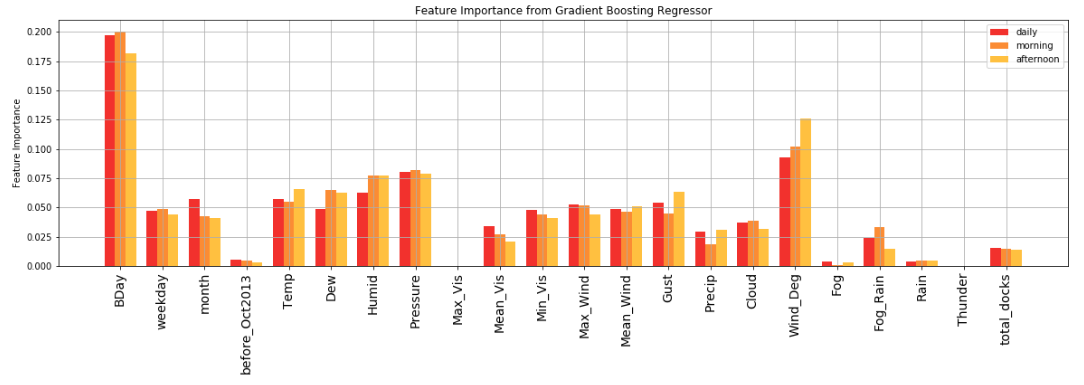
\includegraphics[width=1\textwidth]{RegressorImportance.png}				\caption{\label{fig:regressor_importance}Feature importances for the best regressor.}	
			\end{figure}	
			
			The importances have almost the same distribution among features for the three time periods (daily, am, pm). Strangely the wind degree and pressure are two most important features for the Gradient Boosting Regressor, ranking the second and the third.
			
			\begin{figure}
				\begin{subfigure}[b]{0.4\textwidth}
					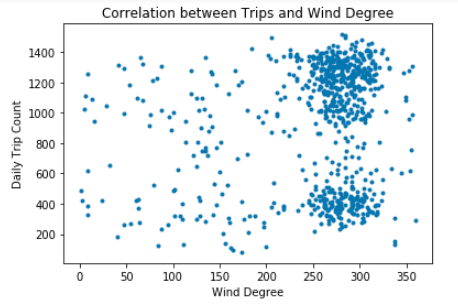
\includegraphics[width=\textwidth]{WindDegree.png}
					\caption{Trip Counts vs. Wind Degree}
					\label{fig:wind_degree}
				\end{subfigure}
					%
				\begin{subfigure}[b]{0.6\textwidth}
					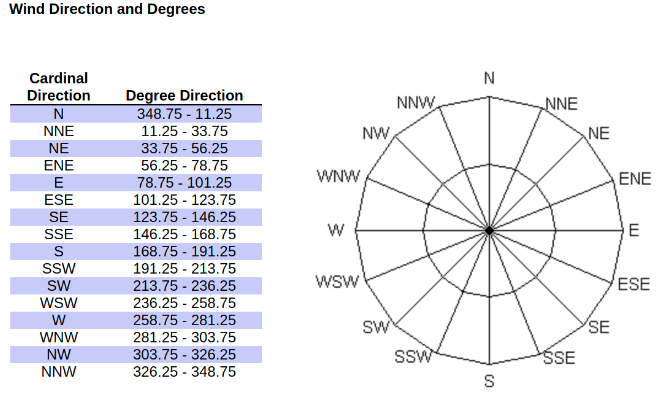
\includegraphics[width=\textwidth]{WindDirection.png}
					\caption{Wind Direction vs. Wind Degree}
					\label{fig:wind_direction}
				\end{subfigure}
				\caption{Wind degree exploration.}
				\label{fig:wind}
			\end{figure}
			
			Plotting the trip counts vs. the wind degree gives Figure \ref{fig:wind_degree}. Most of the data points have wind degrees falling within around 240-320 degrees. This corresponds to wind directions of WSW, W, WNW, NW according to this \href{http://snowfence.umn.edu/Components/winddirectionanddegreeswithouttable3.htm}{source} (see Figure \ref{fig:wind_direction}). So most of the time the wind comes from the north west. No clear linearly relationship is seen here. In fact, the pressure plot shows a similar feature. What is the feature importance really telling us?

			The Gradient Boosting Regressor we used here is essentially a decision tree based model. Its importance can be explained by that for \href{|http://scikit-learn.org/stable/modules/generated/sklearn.tree.DecisionTreeRegressor.html}{decision tree}. 
			
			\begin{leftbar}
				The feature importances. The higher, the more important the feature. The importance of a feature is computed as the (normalized) total reduction of the criterion brought by that feature. It is also known as the Gini importance \href{https://www.stat.berkeley.edu/~breiman/RandomForests/cc_home.htm#varimp}{R255}.
			\end{leftbar}
			
			According to \href{https://datascience.stackexchange.com/questions/16693/interpreting-decision-tree-in-context-of-feature-importances}{this link}:
			
			\begin{leftbar}
				Just because a node is lower on the tree does not necessarily mean that it is less important. The feature importance in sci-kit learn is calculated by how purely a node separates the classes (Gini index).
			\end{leftbar}
			
			So the importance to a decision tree is only judged by whether it reduces the complexity of the tree. This is somewhat disappointing as it is not very helpful in interpreting the results. Nevertheless, at least some really important features that are inherently linked to the daily trip counts must be ranking on the top, such as the business day, the humidity, the temperature, etc.
			
			\subsubsection{Test the Performance Treating the Data as Time Series Data}
			The previous analysis has a presumption that the pattern of the daily trip count does not vary over time given all the available features. This is true to the first approximation: without a big change on the economy and the society during 2013-2015, the behavior of a large group of people are expected to be relatively stable. People get used to things that become a part of their life. Nevertheless, it is more to the essence of the data when treating it as time series data. This is also a good test to challenge the validity of the presumption made earlier. Moreover, this will make the model more practical to guide the real-world operation as we are not able to get data from the future except those that can be forecast. In fact, the power of prediction into the future is what makes machine learning valuable; no cheating is allowed and even possible.
			
			For time-series data, the train test split is not done by shuffling the data and divide it into two parts. The last part of the sorted data by date that happen "in the future" will be separated apart as the testing set. 20\% of the data will be left out, which makes 2015-04-08 as the splitting date. 
			
			The Gradient Boosting Regressor is still used to train the training set. Several rounds of grid searches are done to find the best hyper-parameters. The hyper-parameters used in the final round of the grid search are listed below:
			
			\begin{itemize}
				\item 'learning\_rate': [0.05, 0.06, 0.07]
				\item 'max\_depth': [5, 6, 7]
				\item 'min\_samples\_leaf': [1, 2, 3]
				\item 'n\_estimators': [50, 100, 150]
			\end{itemize}			
			
			Note that the the TimeSeriesSplit is used instead of the shuffle split for cross validation sets generation. The hyper-parameters for the best regressor turn out to be quite different than those used previously. 
			
			The results are interesting. With the median absolute error as the metric, the prediction is worse on the time-series treatment (82.9 vs. 54.5). However, considering the improvement from the benchmark model, it does not seem so bad. The drop in median absolute error from the benchmark model to the best model is about 250 for the time-series treatment, compared to about 210 for the regular treatment. 
			
			If the metric is switched to the root mean square logarithmic error, the prediction on the time-series treated dataset gets a better score not only in the absolute performance, but also in the relative improvement from the benchmark. Although the regressor does a poorer job in predicting trip counts in median values, it seems that the prediction on the general trip counts is better, particularly on those dates that have trip counts distant from the median.
			
			This model is robust shown by the 15-K-Fold cross validation result:
						
			array([ 56.91419936,  62.82644608,  81.42689126,  62.66884854,
					70.48147576,  81.19349047,  56.29945758,  69.14984492,
					62.77203726,  63.43828315,  75.44166919,  55.78103516,
					73.99309373,  66.02656371,  63.09695277])		
			
			It is somewhat safe to conclude that no noticeable information leaking is observed by not splitting the dataset in the time-series approach. The regression problem for daily trip count prediction is time-independent to a large extent: the first approximation is valid. Nevertheless, I will stick to the time-series treatment for the rest of the analysis as it is the ideal scenario for practical use.	
			
			\subsubsection{Decision Tree Display}			
			The feature importances for the time-series split dataset are nearly the same as those of the regularly split dataset. In order to understand more how to utilize the feature importance to interpret the result, one decision tree in the tree group of the Gradient Boosting Regressor is studied below.
			
			\begin{figure}
				\centering
				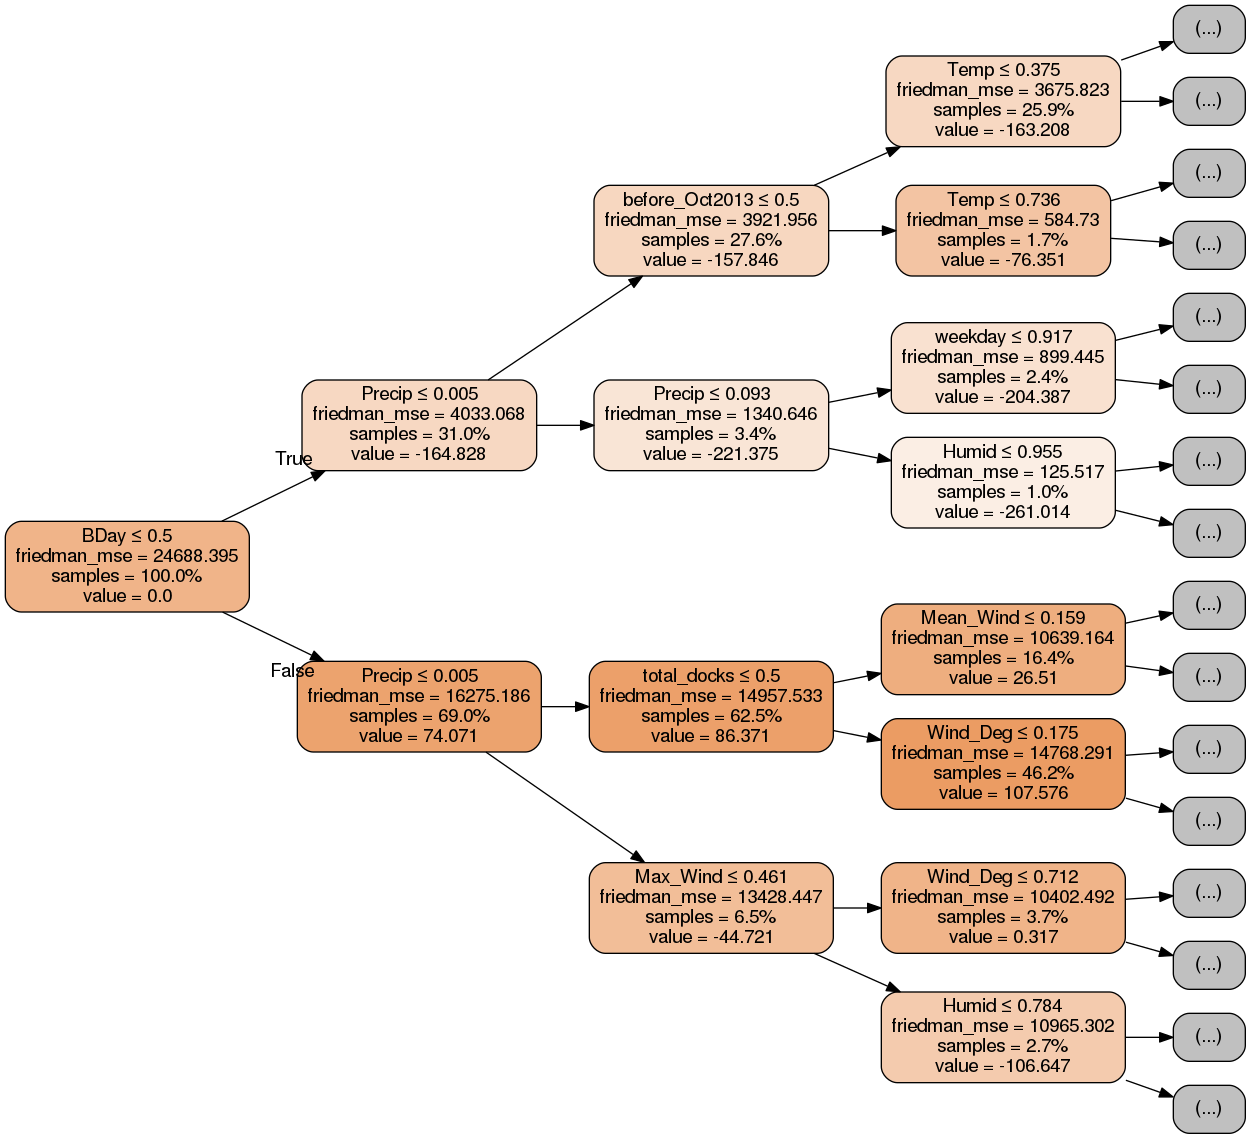
\includegraphics[width=1\textwidth]{sub_tree_16.png}				\caption{\label{fig:sub_tree_16}An instance tree from the Gradient Boosting Regressor.}	
			\end{figure}	
			
			A decision tree is taken from the "estimators" from the regressor. This is one of the 100 estimators. The number of estimators was decided from the grid search process. The tree is display in Figure \ref{fig:sub_tree_16} using graphviz. I choose to display only 3 depths (totally 6) so that most important splitting can be investigated. 
			
			The first splitting point for this tree is the business day. The samples are split to ~70\% in business days, and the rest in non-business days. This is a good start as it increases the information value of the business day samples to 74 from 0, which is a big leap. The higher the information value, the purer the node and the closer to the final conclusion. Following the darker color for the nodes, we can see a clear pattern for trips that happens in a business day with little rain, having less total docks and wind direction more from the southeast. These dates tend to have similar trip counts.
			
			The interpretation from the above seems to be very smooth. This is indeed the power of the decision tree. However, I must point out that the case with a tree-based boosting method is more complicated than a single tree. Remember there are 100 individual decision trees in the Gradient Boosting Regressor. All of them will vote for the final results. The contribution of a specific decision route -- like the example we explored in the last paragraph -- from a single tree is hard to quantify. Another thing to note is that the data were scaled earlier to be suitable to explore all kinds of algorithms, so the splitting point in the tree nodes for a specific feature is not its actual value, but rather the position in its full range. To make better use of the decision tree, the splitting points need to be converted back to its original scales. 
			
			\subsubsection{Feature Importance Ranking}	
			Although an individual tree in the ensemble model gives an idea of how to interpret the result, I am still not confident and comfortable to rely on the tree-based method for the result interpretation. Is there a model that gives not too bad prediction but has a better interpretability? One answer is the linear models.
			
			Let's pick the best performing linear models from the earlier presented regressor contest, the Lasso regressor. Lasso is a linear model with L1 regularization. This model is often used to reduce the dimension of the dataset by identifying unimportant features, so it is a good model to explore. 
			
			A fast search of the optimal parameter for the Lasso can be done with a built-in function in sklearn named LassoCV. With the best Lasso model, the performance on the testing set is worse than the Gradient Boosting Regressor, as expected. This being the fact, this model still does much better than the benchmark, which suggests that it does grab quite some valuable information from the dataset so that we can still use it for rough assessment of the features. 
			
			A similar K-fold cross validation shows the robustness of the Lasso model:
			
			array([ 86.29313305,  94.0246247 ,  95.11989394,  78.22327123,
					85.73315507,  96.94586284,  77.22026939,  79.683902  ,
					85.52358063,  78.78471477,  89.55374939,  77.82806515,
					88.56895503,  75.24744846,  81.60389828]).
			
			Since Lasso is a linear regression method, if all feature columns are normalized to (0, 1), the fitted coefficients become comparable. A feature coefficient can be further adjusted by the center of the most frequently appearing values, i.e. the mean or median. If one feature has most of the values in the low end of its range, the linear regression model tends to assign a larger coefficient to it. Similarly, it one feature has most of the values in the high end, its coefficient tends to be underestimated. So the mean value of a column will be calculated and then multiplied with the coefficient to get the adjusted coefficient.
			
			Considering that only when a feature having nonzero value does it contribute to the final result, the mean of a feature column will be calculated after all zero values are removed from the column before being used for the adjustment. 
			
			\begin{figure}
				\centering
				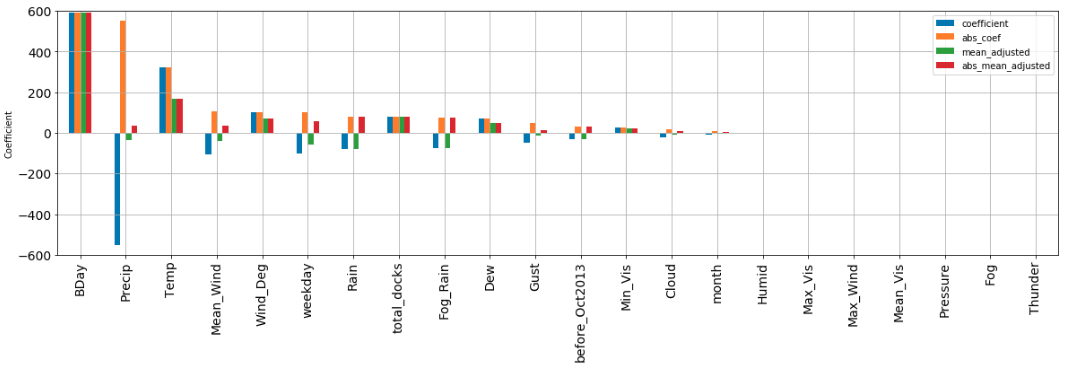
\includegraphics[width=1\textwidth]{LassoImportance.png}				\caption{\label{fig:lasso_importance}Feature importance exploration with Lasso model.}	
			\end{figure}	
			
			Figure \ref{fig:lasso_importance} shows the feature importance ranking from the Lasso model. To assist visual comparison, I also put the absolute values of the original and the mean value adjusted coefficients on the figure. 
			
			Before applying coefficient adjustment, this graph is already making more sense than feature importance for the tree-based regressor. First of all, positive and negative coefficients indicate the corresponding influence of that feature on the final results. For instance, the temperature has a positive coefficient, which means that when the temperature goes higher, there tends to be more trips. This is totally reasonable as the Bay Area is generally not hot over the year; only cold weather will prevent people from riding bikes. Another example is the rain and the precipitation. When there is rain, especially big rain, people will refrain from riding bikes. I summarize features with positive and negative effect below:
			
			\begin{itemize}
				\item Positive: is a business day, higher temperature, larger wind degree (from north, happening in summer), more total docks, higher dew point, better minimum visibility.
				\item Negative: more precipitation, mean higher wind speed, the closer to the end of the week, raining, with fog and rain, higher gust speed, trips before Oct2013 (not long after the stations were installed), more cloud (less sunshine), closer to the end of the year.
				\item Not relevant: humidity, mean and max visibility, max wind speed, sea level pressure, with fog or thunder.
			\end{itemize}
			
			When the mean values are applied for adjustment, the ranking changes a bit. The precipitation becomes a much less important feature, so do the mean wind speed and the max gust speed. Note that the categorical features are robust to this adjustment as they have only 0 or 1 values, always getting the mean value of 1. This does not mean that they are overestimated though. 
			
			The business day is still the most important feature, matching the finding with the tree-based method. However, the importance of the wind degree, for example, has dropped. The sea level pressure even becomes irrelevant. The importance result from the Gradient Boosting Regressor contradict with that from the Lasso. How do we know if the judgment based on the Lasso is reliable? This can be tested by evaluating the dataset with those "irrelevant" feature columns removed.
			
			\subsubsection{How does Irrelevant Feature Removal Impact the Prediction?}
			
			Those feature columns with zero coefficients from the Lasso regressor are removed from the dataset: Humid, Max\_Vis, Max\_Wind, Mean\_Vis, Pressure, Fog and Thunder. Note that the pressure, humidity, max wind speed are ranking in top 10 most important features for Gradient Boosting Regressor.
			
			Amazingly, using the Gradient Boosting Regressor, the performance gets boosted by dropping the "irrelevant" features no matter which metric is used! This is a strong proof that Lasso picked the right ones. It also proves that the result interpretation from the Lasso is reliable.

			\subsubsection{Discussion on the Difficulties and Complications Encountered During the Implementation}

			The complication started to come up from the very beginning of the work. 
			
			At the very beginning of the project, not so many useful features were created or engineered; they developed during the implementation so that the code has to be changed multiple times. 
			
			Initially only the count of daily trip of all stations was of concern until I figured out that the data can be divided into five regions, each with a special pattern. Thus, all the regions had to be studied separately. The separation leads to the conclusion that only the San Francisco data make sense for this project so that I focus only on this region.
			
			I had thought that a smaller time division during a day may give a great impact on the prediction, but it turns out to be a minor effect. This does complicate the project though.
			
			The most challenging part comes from the interpretation of the result. The tree-based method did not give seasonable feature importance ranking. I had attempted to give the result some explanation in order to understand it, including exploring a particular decision tree, but failed. This leads to the exploration of the linear regression method for the interpretation purpose. 			
					
		\subsection{Classfication Problem for Subscriber Type Prediction}
		Subscribers of bike-sharing service are more committed to the program and the frequent users. People subscribe the service, because they think this service make their life easier, i.e. more economic and / or convenient. Subscription is a win-win situation for the users and the company, so one important question is how to persuade people to go for the subscription. If the marketing department of the company gets a budget with an attempt to enlarge the subscriber base, how should they spend it wisely? Without deep understanding the behavior of current non-subscribers, it is difficult to make a proper go-to-market strategy. Below I will explore a solution to find out the behavioral pattern of non-subscribers, interpreting which gives some idea for a better marketing strategy. 
		
			\subsubsection{Benchmark Model}
			
			For the classification problem, no discussion exists to my best knowledge. A plain random guess can serve as the benchmark model. A naive predictor that always predicts a subscriber will be used for the accuracy as most of the labels are subscribers. Another naive predictor that always predicts the non-subscriber will be used for F0.5 score as the metric. A benchmark model should always try to achieve the best score, despite the limited effort and information.
			
			The logistic regression is arguably the most frequently used model for binary classification problem. It will serve as an advanced benchmark model that can be used for both metrics. 
			
			\subsubsection{Feature Data Scaling}
			
			\begin{figure}
				\centering
				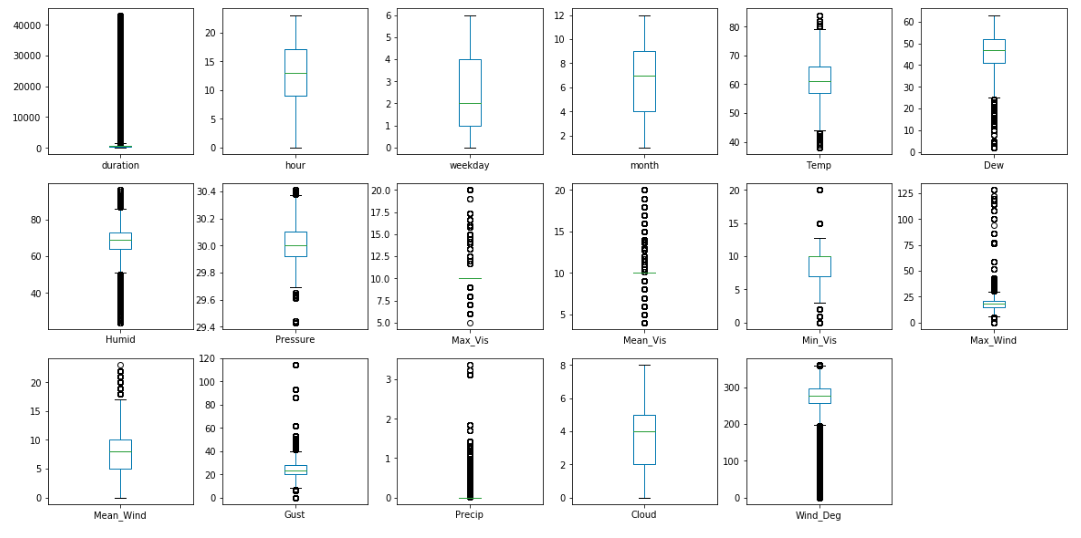
\includegraphics[width=1\textwidth]{FeatureScaleCls.png}				\caption{\label{fig:feature_scale}Explore the value distribution of each feature.}	
			\end{figure}	
			
			\begin{figure}
				\centering
				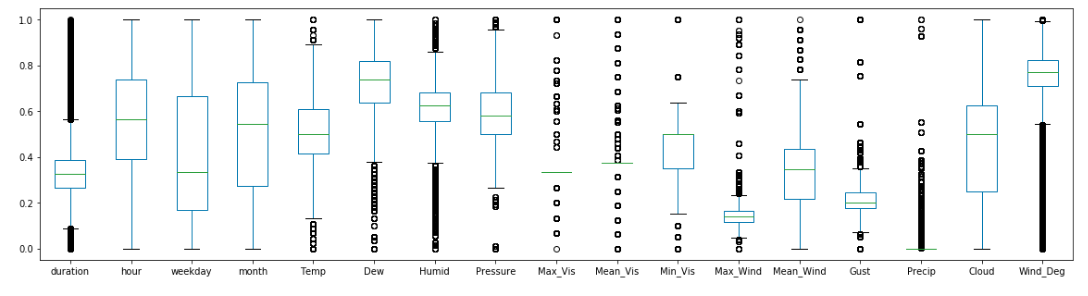
\includegraphics[width=1\textwidth]{FeatureScaled.png}				\caption{\label{fig:feature_scaled}Show the scaled features.}	
			\end{figure}	
			
			Similar with the regression problem, each feature column will be normalized first before further investigation. Figure \ref{fig:feature_scale} shows the data distribution for all the features in the dataset created for the classification problem.
			
	 		This is the box-and-whisker diagram: the bottom and top of the box are the first and third quartiles with the band inside the box the median value. The upper whisker extends 1.5 times the IQR (inter-quartile range) above the third quartile; the lower whisker extends 1.5 times the IQR below the first quartile. This is a good method to view the value distribution within the data.
			 
			Four features seem to have skewed data: the duration, the max wind, the max gust and the precipitation. The max wind and max gust features still have a reasonable range: the median value is more than 10\% of the max value. The precipitation data contain too many values close or equal to zero: this is fine as at least nonzero values don't seem to be very skewed. The real potential trouble maker is the duration. The median value is orders of magnitude far from the max. So logarithm will be first applied to the duration data. After that, all the features will be scaled within the range of 0 and 1. As shown in Figure \ref{fig:feature_scaled}, now the scaled data look more suitable for various machine learning algorithms.
			
			\subsubsection{Generate Training and Testing Sets}
			After proper data scaling, the feature columns and the label column is separated. The label is set to 1 for the non-subscriber and 0 to the subscriber. Then the training and testing sets is split. I still choose to separate out 20\% of the data as the testing set. 
			
			The scoring metric is set to be F0.5 score, which is a variant of the F1 score with more focus on the precision than the recall. It is more helpful to figure out a pattern representing a relatively smaller group of non-subscribers with more confidence, than a pattern for a broader group with low confidence. After all, non-subscribers may have a larger variety in constituents than the subscribers. One should target those having distinct behaviors to the subscribers. If we emphasize the recall rate too much, some characteristics of subscribers will leak into the pattern and make the pattern less representative of the targeted customers.
			
			The cross validation set is also configured here. The stratified K-fold is used as this is an imbalanced dataset with much more subscribers than non-subscribers.
			
			Note the size of the dataset. The training set has 535022 samples and 30 feature columns. The training data is much larger than the one we dealt with for the regression problem. To grab the essence of the dataset and quickly explore promising classifiers, the dataset will be down-sampled as described in the next sub-section.			
			
			\subsubsection{Down-sample the Training Set for Quick Classifier Exploration}
			The principle of the down-sampling is to distill the essence of the data without losing much information. This is done by removing similar feature value combinations in the training set. The assumption is that similar feature value combinations will lead to a similar label.
			
			First, data with different labels are separated to deal with independently. The number of unique values of each column is calculated. Sort the data by columns following the order of uniqueness. The less unique values a column has, the earlier the column will get sorted. 
			
			Once sorted, the squared sum of element-wise difference between adjacent samples is calculated. Only the sample with the squared sum against its neighbor is above the threshold will be kept. Iterate the process until the size of the data doesn't change more than the allowed difference from the previous run.
			
			The threshold is calculated as the squared sum of ensemble deviation. The ensemble deviation is the deviation allowed for one single feature multiplied by the number of numeric features. Zero variation is allowed for all categorical features as they have only two values to vary, 0 and 1. A sample is considered to have enough uniqueness if a single categorical feature is different than another sample even if other features have identical values. Thus, all different combinations of these features will be kept.
			
			A maximal deviation of one feature is set to be 0.03. This means that within a column, two values will be considered to have similar impact on the prediction of the label if the value difference is less than 3\% of the total range from 0 to 1. 
			
			I must admit that this method is not ideal: when comparing two samples, if only one numeric feature changes while the others remain the same, the deviation of that particular feature can be up to 0.51 (there are 17 numeric features) before being considered different. Most likely the duration impact will be weakened due to its value variety: a big range of duration will be considered to have no impact on the label as they lack of uniqueness to the down-sampling method. 
			
			Nevertheless, this down-sample technique gives us a more manageable dataset with a lot of information. The down-sampling process is quick and it compresses the data by 98.1\% to 10354 samples in total. Experiments will be done on this dataset before scaling up to the entire dataset.

			\subsubsection{Explore Proper Classifiers for the Down-sampled Training Set}
			
			\begin{figure}
				\centering
				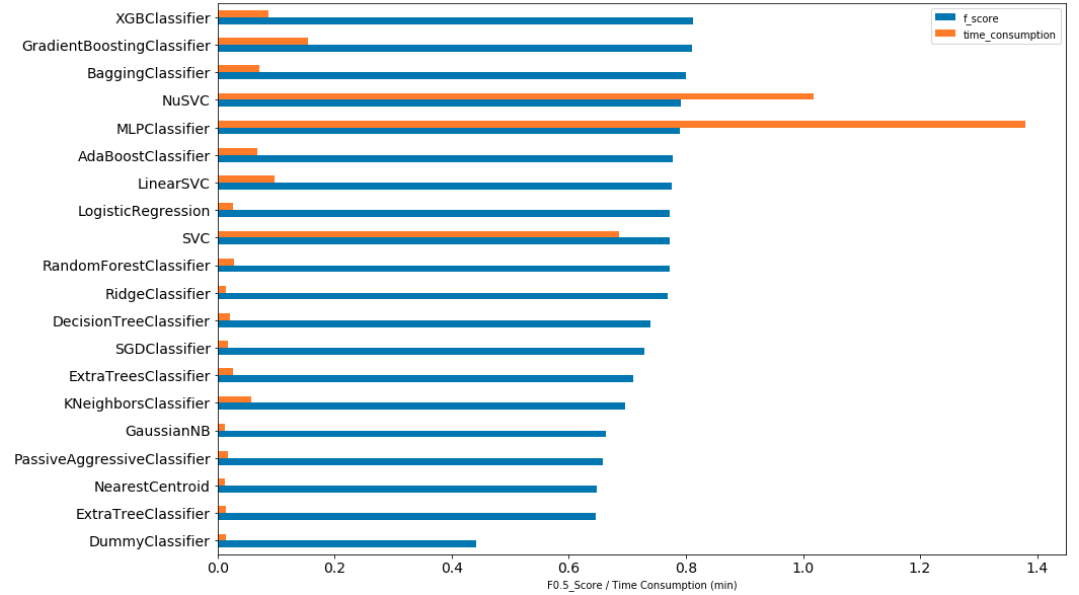
\includegraphics[width=1\textwidth]{Classifiers.png}	\caption{\label{fig:classifiers}Explore the performance and time consumption of classifiers.}	
			\end{figure}	

			All applicable sklearn classifiers plus the xgboost classifier are applied to the down-sampled training set with default settings to give an overview of performance of the frequently-used classifiers. These classifiers are briefly described as follows (mostly from \href{http://scikit-learn.org/stable/supervised_learning.html}{sklearn website}):
			
			\begin{itemize}
				\item XGB Classifier: XGBoost is an implementation of gradient boosted decision trees designed for speed and performance. XGB Classifier is the classifier version of the XGBoost.		
				
				\item Gradient Boosting Classifier: Gradient Boosting for classification. GB builds an additive model in a forward stage-wise fashion; it allows for the optimization of arbitrary differentiable loss functions. In each stage n\_classes\_ regression trees are fit on the negative gradient of the binomial or multinomial deviance loss function. Binary classification is a special case where only a single regression tree is induced.
				
				\item Bagging Classifier: an ensemble meta-estimator that fits base classifiers each on random subsets of the original dataset and then aggregate their individual predictions (either by voting or by averaging) to form a final prediction.
				
				\item Nu SVC: Nu-Support Vector Classification. Similar to SVC but uses a parameter to control the number of support vectors.
				
				\item MLP Classifier: Multi-layer Perceptron classifier. This model optimizes the log-loss function using LBFGS or stochastic gradient descent.
				
				\item Ada Boost Classifier: a meta-estimator that begins by fitting a classifier on the original dataset and then fits additional copies of the classifier on the same dataset but where the weights of incorrectly classified instances are adjusted such that subsequent classifiers focus more on difficult cases.
				
				\item Linear SVC: Linear Support Vector Classification.
				
				\item Logistic Regression: a linear model for classification rather than regression. In this model, the probabilities describing the possible outcomes of a single trial are modeled using a logistic function.
				
				\item SVC: C-Support Vector Classification.	The implementation is based on libsvm.
				
				\item Random Forest Classifier: a meta estimator that fits a number of decision tree classifiers on various sub-samples of the dataset and use averaging to improve the predictive accuracy and control over-fitting.
				
				\item Ridge Classifier: a classifier using Ridge regression.
				
				\item Decision Tree Classifier: a decision tree classifier.
				
				\item SGD Classifier: this estimator implements regularized linear models with stochastic gradient descent (SGD) learning: the gradient of the loss is estimated each sample at a time and the model is updated along the way with a decreasing strength schedule (aka learning rate). 
				
				\item Extra Trees Classifier: this class implements a meta estimator that fits a number of randomized decision trees (a.k.a. extra-trees) on various sub-samples of the dataset and use averaging to improve the predictive accuracy and control over-fitting.
				
				\item K-Neighbors Classifier: a classifier implementing the k-nearest neighbors vote.
				
				\item Gaussian NB: it implements the Gaussian Naive Bayes algorithm for classification. The likelihood of the features is assumed to be Gaussian.
				
				\item Passive Aggressive Classifier: the passive-aggressive algorithms are a family of algorithms for large-scale learning. They are similar to the Perceptron in that they do not require a learning rate. 
				
				\item Nearest Centroid: each class is represented by its centroid, with test samples classified to the class with the nearest centroid.
				
				\item Extra Tree Classifier: Extra-trees differ from classic decision trees in the way they are built. When looking for the best split to separate the samples of a node into two groups, random splits are drawn for each of the max\_features randomly selected features and the best split among those is chosen. Note that this is different than the Extra Trees Classifier which is an ensemble method.
				
				\item Dummy Classifier: a classifier that makes predictions using simple rules. The default strategy is 'stratified' which generates predictions by respecting the training set’s class distribution.
			\end{itemize}
			
			Considering the size of the data, I not only score each classifier on their performance with F0.5 score, but also record the time consumption for each classifier. For a large dataset, a slow algorithm may not be a good choice when it comes to hyper-parameter tuning. That being said, performance may be the utmost important criterion for certain data exploration. For this study, as we only need to qualitative grasp on the non-subscriber pattern, it is not wise to start with time-consuming models. The result is shown in Figure \ref{fig:classifiers}.
			
			Finding a balance between a high score and a shorter training time is an art. I will follow these strategies:
			
			\begin{enumerate}
				\item Classifiers performing better than the average will stay.
				\item Normalize the F0.5 score on the good classifier group to exaggerate the score difference among classifiers.
				\item Craft a formula to balance the performance and the time consumption with more emphasis on the performance.
				\item Make sure two of the three top performing classifiers also rank in the top three following the new criterion.
			\end{enumerate}
							
			\begin{table}
				\centering
				\begin{tabular}{ l r }
					XGBClassifier              &   11.465292 \\
					BaggingClassifier          &   8.745233 \\
					RidgeClassifier            &   7.770470 \\
					GradientBoostingClassifier &   6.113944 \\
					LogisticRegression         &   5.468275 \\
					RandomForestClassifier     &   4.841627 \\
					AdaBoostClassifier         &   2.737575 \\
					LinearSVC                  &   1.720470 \\
					NuSVC                      &   0.414178 \\
					MLPClassifier              &   0.287001 \\
					SVC                        &   0.194940 \\
					DecisionTreeClassifier     &   0.088574 \\
					SGDClassifier              &   0.000000	
				\end{tabular}				
				\caption{Ranking of classifiers.\label{cls_ranking}}
			\end{table}
			
			I will choose the top three classifiers by the ranking (Table \ref{cls_ranking}): XGBClassifier, BaggingClassifier, RidgeClassifier. The LogisticRegression is also chosen as a high-performance benchmark model.
			
			Interestingly, even when this criterion gives so much high emphasis (cubic) on the performance, the Gradient Boosting Classifier still doesn't get into the top three while it was in the top three: it does not have a good performance-effort balance. On the other hand, the RidgeClassifier and the LogisticRegression get to move to the top due to the much less consumption of time.
			
			Down-sampling the training set undoubtedly helps with excluding those classifiers that are too time-consuming. It also gives an idea of the best-performing classifiers. We will check later if a good classifier will do well on both the full dataset and the downsized dataset.
			
			\subsubsection{Find the Optimal Hyperparameters on the Down-sampled Training Data}
			
			\paragraph{For Sklearn Classifiers}
			First the sklearn classifiers are explored. The XGBClassifier will be treated slightly differently and will be investigated later.
			
			To save time in exploring different hyper-parameters for the data, randomized search is used instead of grid search. Note that the number of estimators for the ensemble method (BaggingClassifier here) should not be set to a very large value from its default. The training time scales up very rapidly upon more estimators, while the performance does not get improved significantly.
			
			The hyper-parameters used in the randomized search are:
			
			\begin{itemize}
				\item For BaggingClassifier: {'n\_estimators':[10, 30, 50], 'max\_samples':[0.4, 0.5, 0.6, 0.7]}
				\item For LogisticRegression: {'penalty': ['l1', 'l2'], 'C': np.linspace(0.1, 1.0, 10)} 
				\item For RidgeClassifier: {'alpha': np.linspace(0.1, 1.0, 20)} 
			\end{itemize}
			
			The BaggingClassifier gets a F0.5 score 0.817 (1.5 min), the LogisticRegression 0.774 (50 s) and the RidgeClassifier 0.769 (7 s). The performance increases as a sacrifice in the training time.
			
			\paragraph{For XGBClassifier}	
			The xgboost is a very popular machine learning algorithm recently. It demonstrates very good performance with reasonable training time. Moreover, it can leverage the power of GPU. A quick test on my PC shows a boost of speed at least 4 times on GPU than on CPU.
			
			XGBClassifier has more parameters that can be trained than other ensemble classifiers like the Gradient Boosting Classifier. A good \href{https://www.analyticsvidhya.com/blog/2016/03/complete-guide-parameter-tuning-xgboost-with-codes-python/}{reference} about how to train the XGBClassifier step by step is found on the internet. I also find its \href{http://xgboost.readthedocs.io/en/latest/model.html#}{official website} quite helpful.
			
			To be comparable with other classifiers, the same metric should be used. Unfortunately F beta score is not a default metric / evaluation method for XGBClassifier. A customized evaluation function for the xgboost cross validation is defined (xgb\_f\_score).
			
			Below are the steps that I follow to train the optimal XGBClassifier:
			
			\begin{enumerate}
				\item Fix learning rate and number of estimators for tuning tree-based parameters
				
				\item Tune max\_depth and min\_child\_weight. Grid search {'max\_depth': range(3,10,2), 'min\_child\_weight': range(1,6,2)} and then {'max\_depth':[6,7,8], 'min\_child\_weight':[4,5,6]}.
				
				\item Tune gamma. Grid search {'gamma':[i/10.0 for i in range(0,5)]}.
				
				\item Tune subsample and colsample\_bytree. Grid search {'subsample':[i/10.0 for i in range(6,10)], 'colsample\_bytree':[i/10.0 for i in range(6,10)]}.
				
				\item Tune regularization parameters. Grid search {'reg\_alpha':[0.01, 0.1, 1, 10], 'reg\_lambda':[0.01, 0.1, 1, 10]} and then {'reg\_alpha':[0.5, 1, 2, 3], 'reg\_lambda':[0.5, 1, 2, 3]}.
				
				\item Tune scale\_pos\_weight for balancing the positive and negative weight. Grid search {'scale\_pos\_weight': np.linspace(0.1, 1, 10)}.
				
				\item Optimize the learning rate.				
			\end{enumerate}
			
			To tune parameters, first try coarse steps for the grid search. If significant performance is observed, another round with a finer step will be investigated. XGBClassifier has a great build-in tool to find out the best number of estimators. This function will be invoked whenever a significant improvement is found by tuning other parameters. 
	
			\begin{figure}
				\begin{subfigure}[b]{0.33\textwidth}
					\centering
					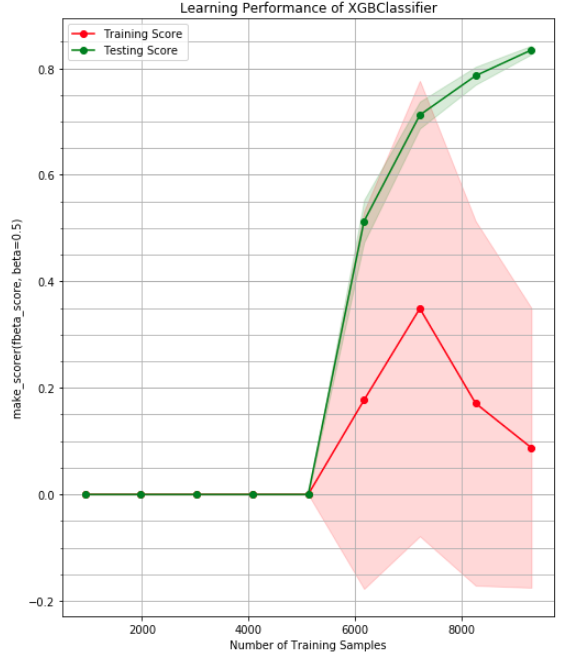
\includegraphics[width=1\textwidth]{xgbLearningCurve.png}\caption{\label{fig:xgb_lc}Mean of all values.}
				\end{subfigure}
				%
				\begin{subfigure}[b]{0.33\textwidth}
					\centering
					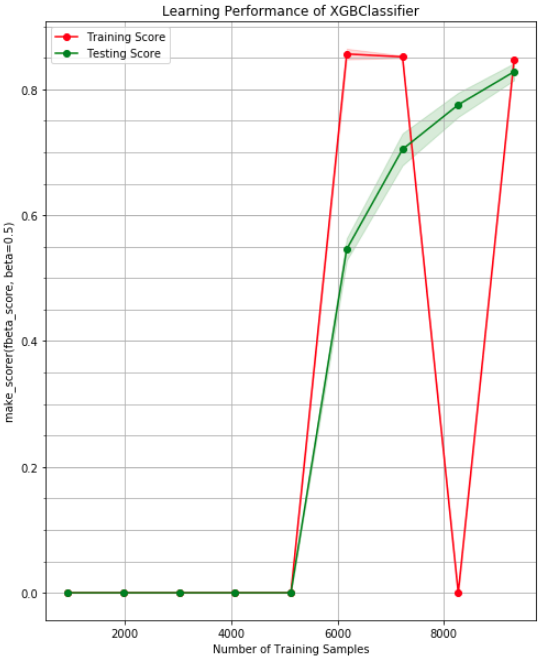
\includegraphics[width=0.96\textwidth]{xgbLearningCurve2.png}\caption{\label{fig:xgb_lc2}Mean of nonzero values.}
				\end{subfigure}
				%
				\begin{subfigure}[b]{0.33\textwidth}
					\centering
					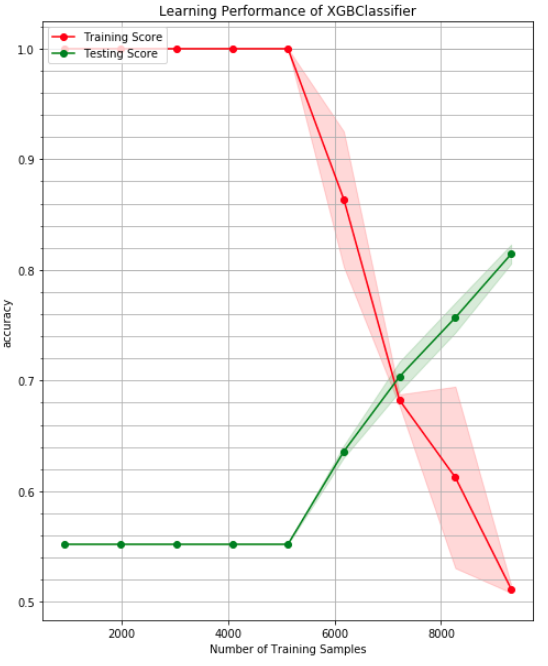
\includegraphics[width=0.96\textwidth]{LearningCurveAcc.png}\caption{\label{fig:xgb_lc3}Accuracy as the metric.}
				\end{subfigure}				
				\caption{The learning curve of the XGBClassifier on down-sampled training set.}
				\label{fig:lcs}
			\end{figure}			
			
			The down-sampled dataset has much fewer samples than the entire dataset. It is necessary to find out whether there are enough data samples for the training or not. Thus, a learning curve is plotted with the best XGBClassifier, shown in Figure \ref{fig:xgb_lc}. The y axis is the F0.5 score. When no positive label is predicted, the F0.5 score value is set to 0. Each data point is the mean value of all cross validation results. The colored area covers one standard deviation from the averaged data points. The red dots are the scores on the training set, while the green dots are on the cross validation set. 			
			
			It is very interesting to see how many training samples are required in order to obtain good performance on the F0.5 score. In fact, the F0.5 score seems to going up even all the samples are used. So some optimization may be required on the entire dataset.
			
			The behavior of the training score is quite strange though. When the mean of all train scores is calculated, the Figure \ref{fig:xgb_lc} is observed which is rather puzzling: the small training score with more samples and the large deviation. When the testing score shoots high, the training score goes to the bottom. Later I find that the training scores is a very sparse array with most of the values to be zero. When the plot\_learning\_curve function is tweaked a bit to take the average of all nonzero, the Figure \ref{fig:xgb_lc2} is observed. The F0.5 score actually does not get too bad when there are nonzero scores. This is probably caused by the low accuracy score with more samples (Figure \ref{fig:xgb_lc3}). Note that these three figures are not referring to exactly the same learning curve. Although the random state of the learning curve cross validation and the classifier is controlled, the randomness still exists somewhere.
			
			Anyhow it is still very strange. Does the XGBClassifier attempt to "underfit" the training set in order to "overfit" the validation set? I could not find an answer to it.
			
			\subsubsection{Evaluate the Classifiers on the Entire Dataset}
			Before applying the XGBClassifier on the entire dataset, remember to set the GPU tree method to 'gpu\_hist' from 'gpu\_exact'. It is faster to train a small dataset with the 'gpu\_hist' method, but it is opposite when it comes a large dataset. A speed improvement can be observed by using the right method on the entire dataset.
			
			\begin{figure}
				\centering
				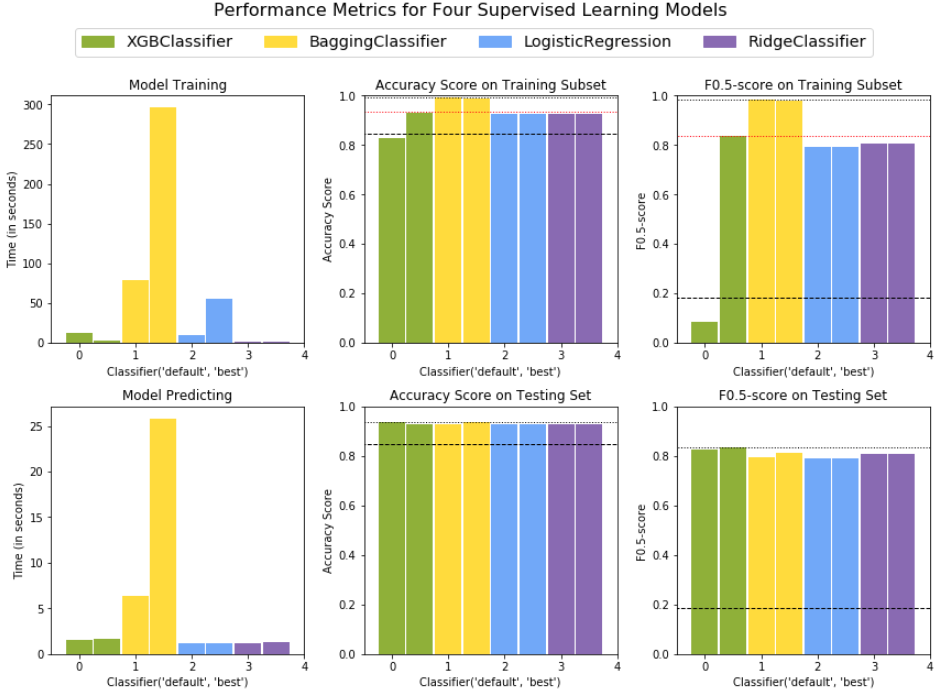
\includegraphics[width=1\textwidth]{ClassifiersPerformance.png}\caption{\label{fig:classifiers_performance}Visualize the performance of classifiers with default and optimized settings.}	
			\end{figure}	
			
			Figure \ref{fig:classifiers_performance} visualizes the performance of the four classifiers chosen for further exploration. The first row shows the performance on the training, while the second row shows it on the testing. 
			
			On the first column, the model training and predicting times are plotted. The BaggingClassifier is the most time-consuming algorithm, while the RidgeClassifier does the best on this. XGBClassifier is doing very well, thanks to the GPU.
			
			On the second column, the accuracy score is calculated on the training set (I set it to the full set) and the testing set. All classifiers are have almost the same score on the testing set no matter how good they are doing on the training set. The black dashed line indicates the accuracy of a naive predictor that always predicts the subscriber. This serves as a benchmark for the accuracy. The black dotted lines on both figures mark the highest score within the figure. The red dotted line on the training figure indicates the highest score on the testing set as a comparison. Interestingly, the XGBClassifier with the default setting does not do a good job on the entire dataset, even worse than the naive predictor. It may not get picked up if the entire dataset was used for classifier filtering.
			
			The third column shows the results with the F0.5 metric. This is the most important column. Clearly, we see that XGBClassifier is the winner on the testing set. BaggingClassifier is doing almost perfect on the training set, but worse in the testing set: it is apparently overfitting the training set. All three classifiers are doing better than the LogisticRegression, the better-performing benchmark model. The XGBClassifier, again, gives some surprise. With the default setting, it get a much lower score on the training set than the naive predictor which always predicts the non-subscriber.
			
			To summarize, in terms of the overall performance, the XGBClassifier is no doubt the best. The RidgeClassifier ranks the third in F0.5 score, but the training and the predicting are pretty quick. The LogisticRegression is doing so-so as a benchmark classifier. The BaggingClassifier takes too much time for the training and the predicting. Also it tends to overfit. Not a good classifier. 

			It is noteworthy that the classifier trained on the down-sampled training set is doing at least no worse than the same classifier with the default setting on the full testing set. Note that the testing set is about ten times the size of the down-sampled training set. This is a good sign that the down-sampling method works to some extent. The down-sampled training set reflects on many aspects of the pattern in the entire dataset. 
		
			\subsubsection{Optimize the Best Classifiers on the Entire Dataset}			
			As we see in the previous sub-section, the XGBClassifier and the RidgeClassifier are the two classifiers that worth further exploration.
			
			\paragraph{Optimizing the XGBClassifier}
			Here are my experience in training the XGBClassifier on the full training set, which is larger and more complex:
			
			\begin{itemize}
				\item The max\_depth will be deeper / larger number.
				\item The learning rate is smaller.
				\item The number of estimator tends to be larger. Don't set that too high, otherwise the training speed is slower (scaling up linearly).
				\item The scale\_pos\_weight is an important parameter for imbalanced data, which is typical. Always use the stratified K-fold for the cross validation so that different splits of data will be similarly imbalanced.
				\item The gamma tends to be smaller.
				\item The subsample and colsample\_bytree become more important.
				\item The reg\_alpha and reg\_lambda values can have more possibility, rather than just the plain 0 or 1.
				\item If the data is extremely imbalanced, max\_delta\_step should be tuned.
			\end{itemize}
			
			\begin{figure}
				\begin{subfigure}[b]{0.49\textwidth}
					\centering
					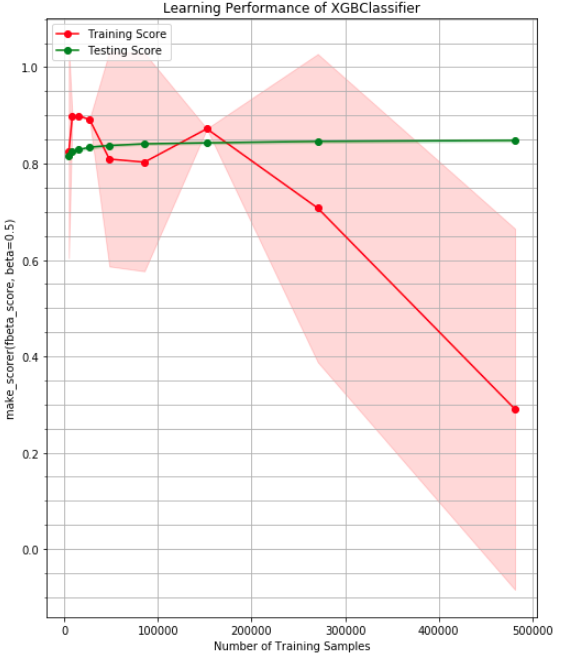
\includegraphics[width=1\textwidth]{xgbFullLearningCurve.png}\caption{\label{fig:xgb_full_lc}XGBClassifier.}
				\end{subfigure}
				%
				\begin{subfigure}[b]{0.51\textwidth}
					\centering
					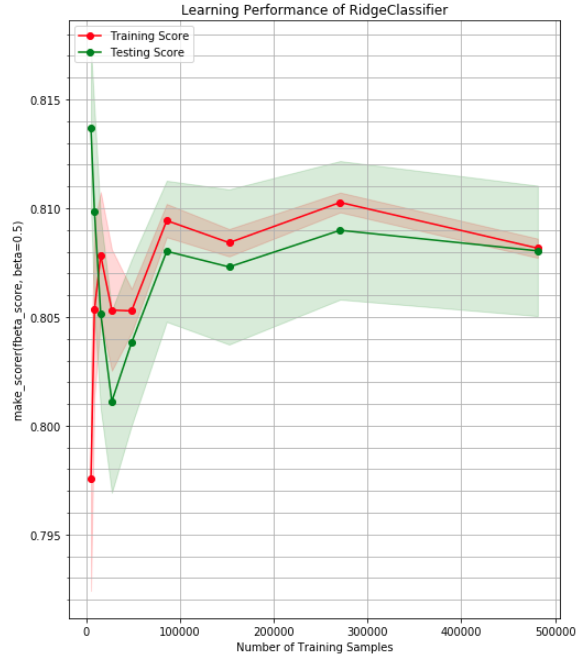
\includegraphics[width=1\textwidth]{RidgeLearningCurve.png}\caption{\label{fig:ridge_lc}RidgeClassifier.}
				\end{subfigure}				
				\caption{The learning curves on the full-size training set.}
				\label{fig:lc_full}
			\end{figure}					
			
			The learning curve of the XGBClassifier is plotted in Figure \ref{fig:xgb_full_lc}. Again, its behavior is quite strange. While the testing score keeps going up to ~ 0.85, the training score is doing some funny walk. 
			
			The robustness of the model is shown by running K-Fold cross validation. The result from a stratified 10-K-Fold cross validation shows the good robustness of the XGBClassifier:
			
			array([ 0.84897667,  0.84544921,  0.8489922 ,  0.85153048,  0.84355132,
			0.85169821,  0.85175132,  0.84633716,  0.84823164,  0.84293689]).
			
			\paragraph{Optimizing the Ridge Classifier}
			The alpha is optimized for the RidegClassifier by two-round grid searches: {'alpha': np.linspace(0.1, 1.0, 5)} and then {'alpha': np.linspace(0.8, 1.0, 5)}. Note that the RidgeClassifierCV cannot be used as it will report an error for the F0.5 score.			
			
			While the XGBClassifier is having a weird learning curve, the optimized RidgeClassifier has a more reasonable learning curve: there is a trend that the training score and the testing score converge to the same when the size of the dataset gets larger. 
			
			This model is also very robust as shown by the cross validation result:
			
			array([ 0.8105724 ,  0.80803687,  0.80862226,  0.81010509,  0.80699701,
			0.81002971,  0.80848105,  0.80346593,  0.81207098,  0.8020107 ]).
			
			\subsubsection{Prediction on the Testing Set}
			Now that the two classifiers have been optimized. Their performance will be tested on the testing set. Here are the results:
			
			\begin{itemize}
				\item The F0.5 score on the testing set with trained model from the downsampled dataset is 0.8354.
				\item The F0.5 score on the testing set with the optimized XGBClassifier on the full-size training set is 0.8519.
				\item The F0.5 score on the testing set with the optimized RidgeClassifier on the full-size training set is 0.8073.
			\end{itemize}
			
			The performance of the XGBClassifier gets a big improvement by training the classifier further on the full-size training set, from 0.8354 to 0.8519. 
			
			\begin{figure}
				\begin{subfigure}[b]{0.57\textwidth}
					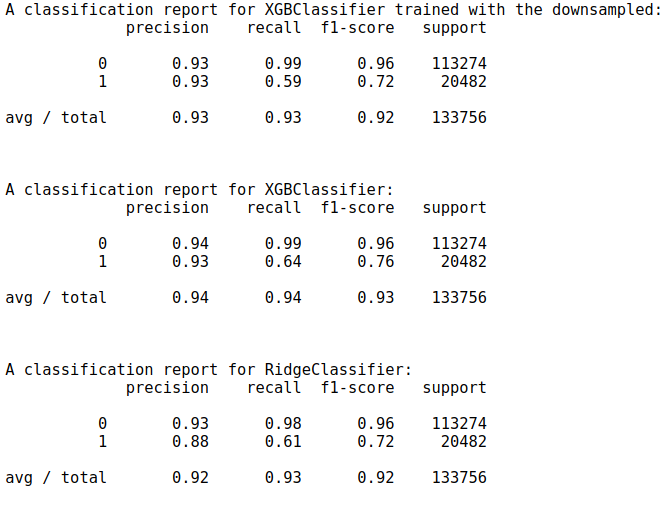
\includegraphics[width=1\textwidth]{ClassificationReports.png}
					\caption{\label{fig:cls_report}Classification reports.}
				\end{subfigure}					
				%
				\begin{subfigure}[b]{0.43\textwidth}
					\centering
					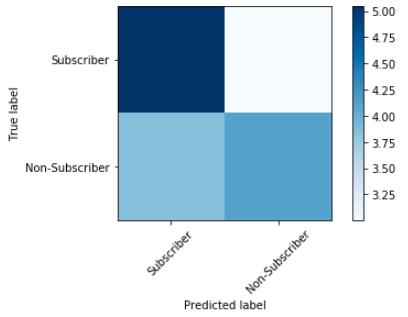
\includegraphics[width=1\textwidth]{ConfusionMatrix.png}\caption{\label{fig:confusion_matrix}Confusion matrix for XGBClassifier (log10 scale).}	
				\end{subfigure}
				\caption{Classification reports and the confusion matrix.}
				\label{fig:confusion_report}
			\end{figure}	
			
			A classification report reveals more details about the performance. In Figure \ref{fig:cls_report}, the precision and the recall of the label 1 (the non-subscriber) are of particular interests. The XGBClassifier trained on the down-sampled training data are doing as well as the one trained on the entire training data in the precision. The latter has an improved F score due to an improvement of the recall. The RidgeClassifier, though with inferior performance in F0.5 score, is not doing bad on the recall. In fact, if F1 score is used as the metric instead, the performance of the RidgeClassifier is as good as the XGBClassifier trained on the down-sampled.
			
			The confusion matrix (Figure \ref{fig:confusion_matrix}) of the optimized XGBClassifier gives an intuitive view on the classification report; the log10 scale is used to magnify the difference. Clearly, we can see that the True Negative to the top left corner has the most samples; the True Positive to the bottom right ranks the second. The color of the False Negative to the bottom left is even lighter and the False Positive to the top right is almost white (least samples). The precision is proportional to the weight of the True Positive on the right column, while the recall is proportional to that on the bottom row. From the color darkness, we can see that precision should be higher than recall, which matches the observation in the classification report.
			
			\subsubsection{Explore Feature Importances}
			\paragraph{Plot XGBClassifier Importances.}
			
			\begin{figure}
				\centering
				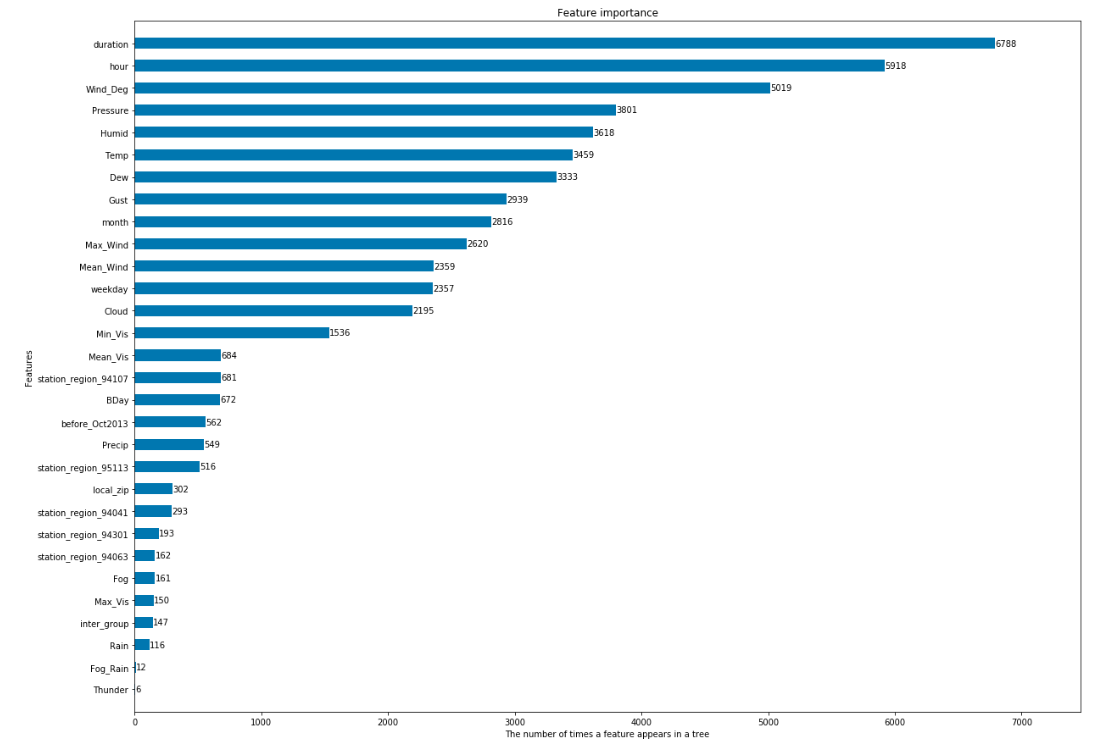
\includegraphics[width=1\textwidth]{xgb_Importance.png}
				\caption{\label{fig:xgb_importance}Feature importance from XGBClassifier.}	
			\end{figure}	
			
			\begin{figure}
				\centering
				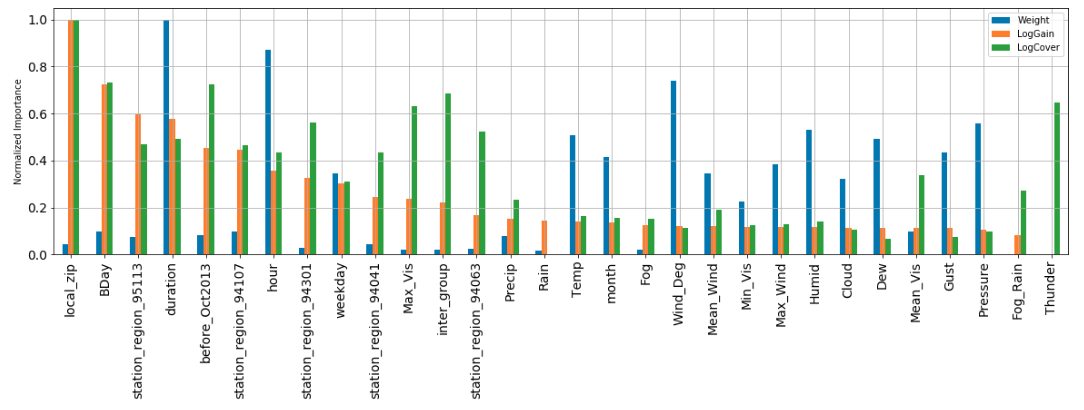
\includegraphics[width=1\textwidth]{Importances.png}
				\caption{\label{fig:importances}All three feature importance types from XGBClassifier sorted by the Gain type.}	
			\end{figure}	

			As usual, the feature importance is plotted to show the ranking (Figure \ref{fig:xgb_importance}). However, when I explore the other two importance types, the gain and the cover, different rankings appear (Figure \ref{fig:importances}). Different importance types are described from the \href{http://xgboost.readthedocs.io/en/latest/python/python_api.html}{xgboost website}:
			
			\begin{leftbar}
				\begin{itemize}
					\item ‘weight’ - the number of times a feature is used to split the data across all trees. 
					\item ‘gain’ - the average gain of the feature when it is used in trees 
					\item ‘cover’ - the average coverage of the feature when it is used in trees
				\end{itemize}				
			\end{leftbar}
			
			The feature importances with the 'gain' and the 'cover' are first scaled logarithmically. Then all three are normalized to have values between 0 and 1 so that they are directly comparable to some extent. Since usually the gain is used to rank the importance, I sort the gain importance in the descending order. 

			One must be very cautious in trusting the importance ranking from XGBClassifier or other tree-based ensemble algorithms. One type's meat is another type's poison. For example, both the 'Gain' and 'Cover' methods select the local zipcode as the most important feature, but it is a very irrelevant feature with the 'Weight'. While the thunder feature almost means nothing to both the 'Gain' and 'Weight', it is a very important feature for the 'Cover'.
			
			This is not yet clear which ranking makes more sense. I will compare all of them with a linear model later.
			
			\paragraph{Display a Decision Tree.}

			\begin{figure}
				\centering
				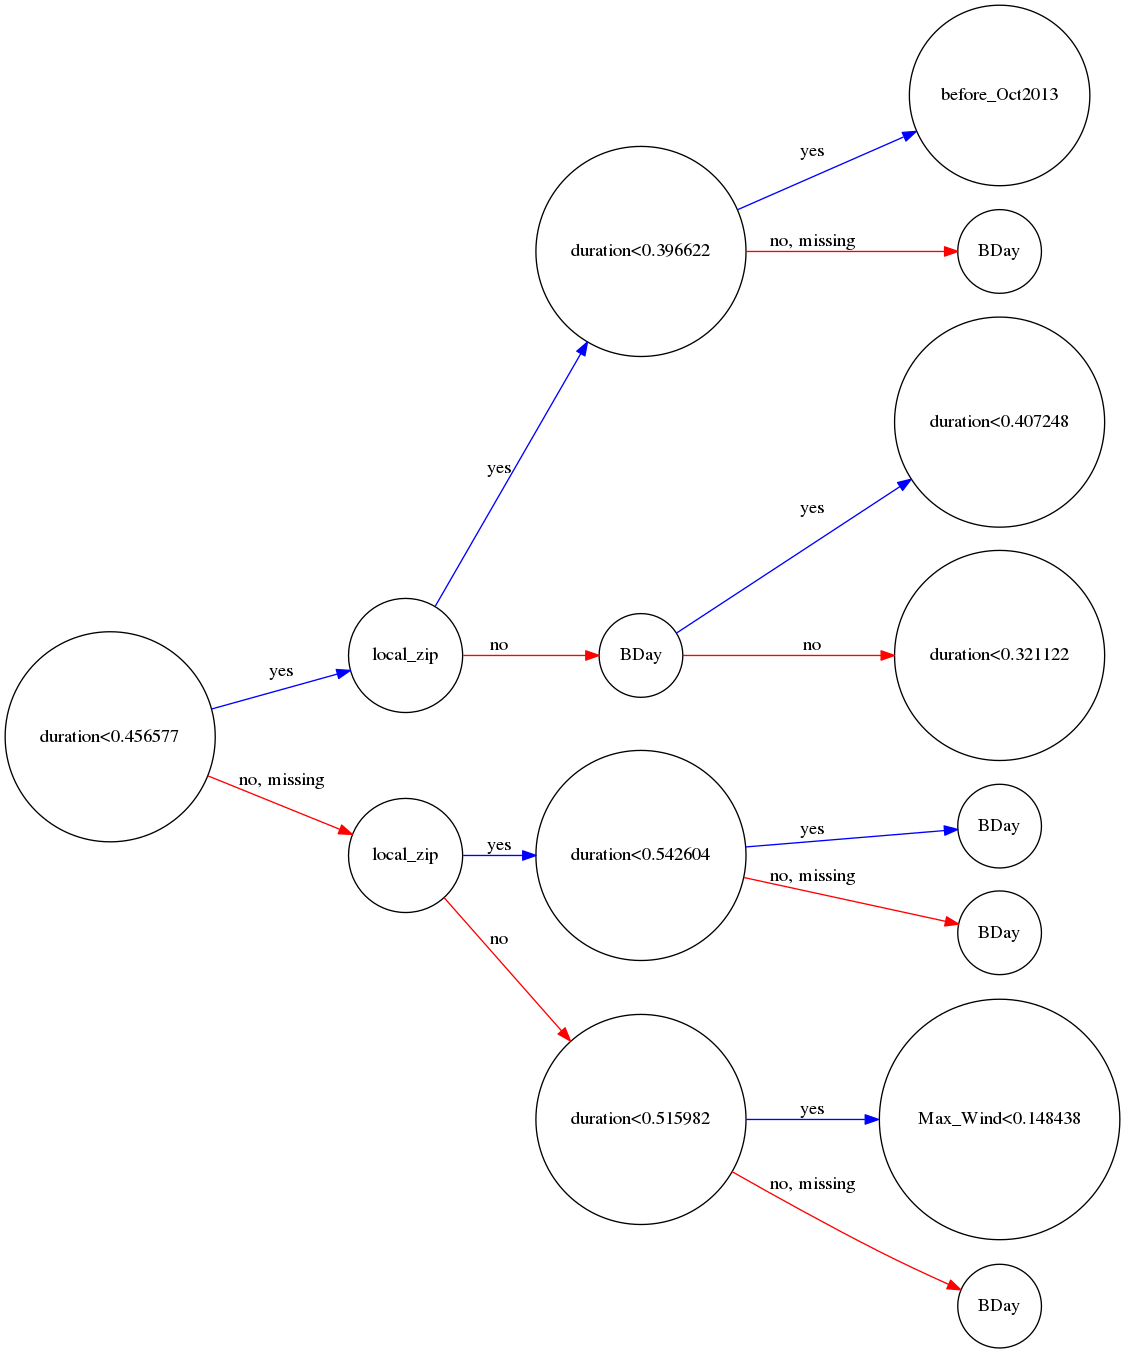
\includegraphics[width=1\textwidth]{xgb_tree_16.png}
				\caption{\label{fig:xgb_tree}An example of decision tree from the XGBClassifier truncated beyond depth 3.}	
			\end{figure}
			
			One estimator (a decision tree) of the XGBClassifier is shown in Figure \ref{fig:xgb_tree}. Only the tree down to depth 3 (totally 9) is shown by modifying the graphviz output (a DOT source code) from the XGBClassifier. This tree is not easily interpretable. The duration and the BDay features are used multiple times; more are anticipated when the tree grows deeper. These two features are important for the tree, but not so intuitive to tell the story. A tree can get deeper for better prediction, but the interpretability is sacrificed.
			
			\paragraph{Explore Important Splitting Points for Important Features.}
			Fortunately, XGBClassifier offers another tool that can help us understand more about the underlying pattern of the data, that is the split value histogram. This function returns how often a split value is invoked for all the estimators. From there, we can figure out one or two most important split values for a feature.		
			
			\begin{figure}
				\centering
				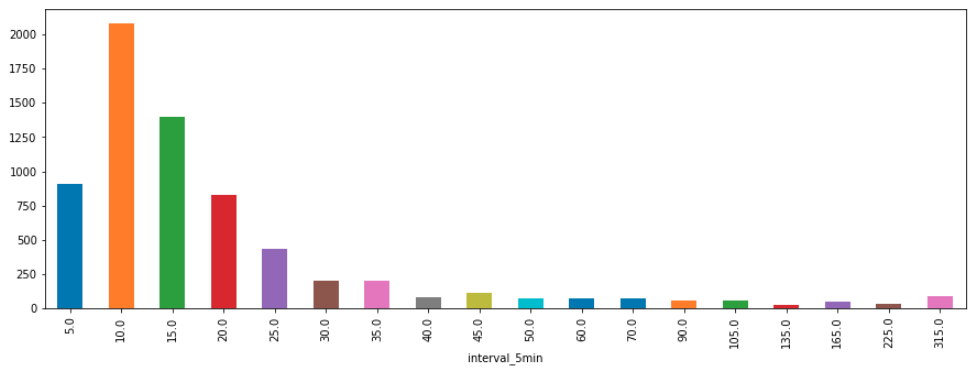
\includegraphics[width=0.8\textwidth]{DurationSplit.png}
				\caption{\label{fig:duration_split}The splitting points for duration feature with 5 min as a step.}	
			\end{figure}
			
			\begin{figure}
				\centering
				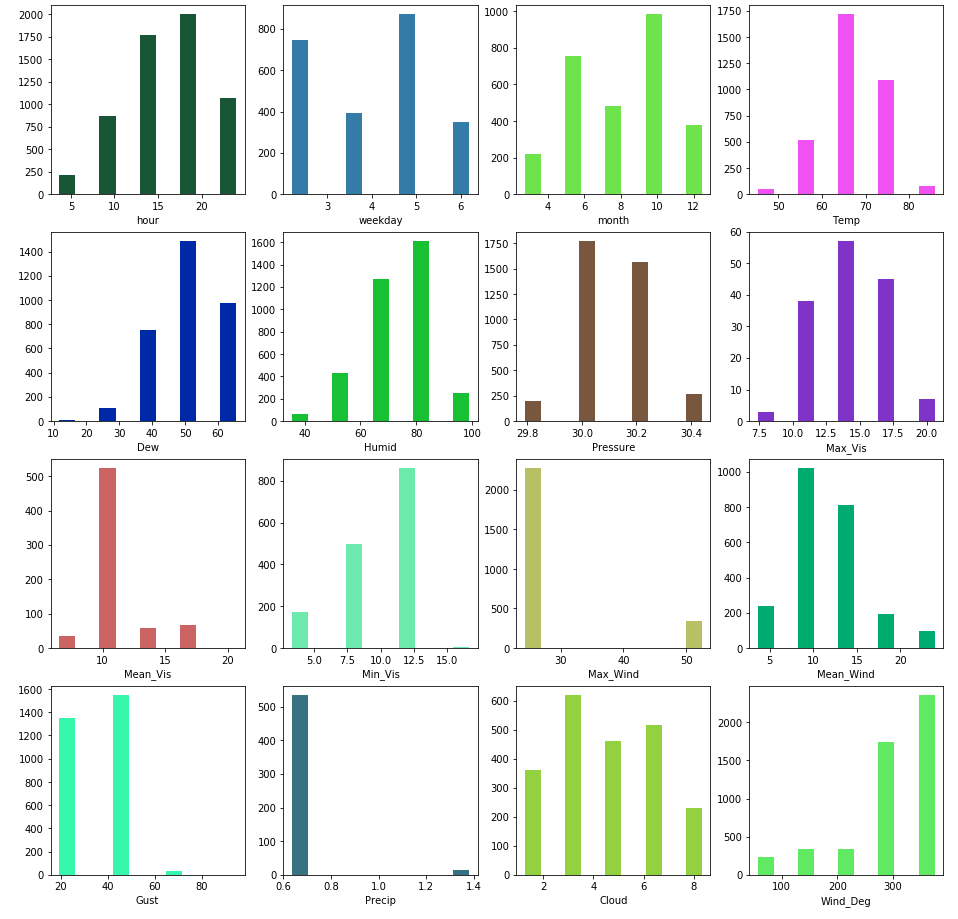
\includegraphics[width=1\textwidth]{FeatureSplit.png}
				\caption{\label{fig:feature_split}Splitting histograms for all features except the duration.}	
			\end{figure}
			
			The data used for the training are scaled to be within 0 and 1. The duration feature was even treated by logarithm before the normalization. To take the advantage of the histograms, we need to transform the data back to its original scale, the real-world values. 
			
			First, the duration feature is scaled back and applied the exponential function to revert the logarithm. Then I break all the duration data into 5-minute slots for easier interpretation. Figure \ref{fig:duration_split} shows that the most frequenly used split point for the duration is at 10 min. This is a hint that either a subscriber or a non-subscribers prefers to use the share-bike for more than 10 minutes at certain conditions.
			
			Splitting histograms of other features are plotted in Figure \ref{fig:feature_split}. Up to 5 division points are allowed for each feature. As a quantitative approach, this could be complementary to qualitative analysis to strengthen the decision making process. Once important features are selected from the qualitative analysis, those features can be explored further by looking at the most frequently used split points.
			
			\paragraph{Feature Importance vs. Feature Uniqueness.}
			\begin{figure}
				\begin{subfigure}[b]{0.5\textwidth}
					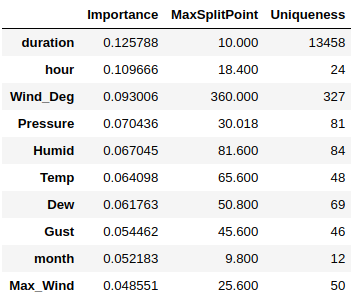
\includegraphics[width=0.9\textwidth]{ImportanceSplitUniqueness.png}
					\caption{\label{fig:importance_split}Top 10 important features by weight.}
				\end{subfigure}					
				%
				\begin{subfigure}[b]{0.5\textwidth}
					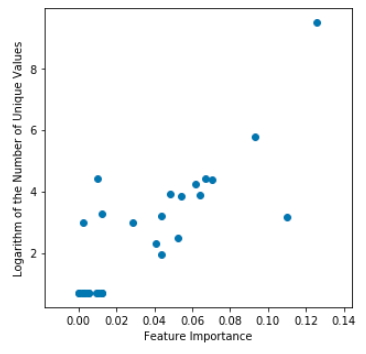
\includegraphics[width=0.8\textwidth]{ImportanceUniqueness.png}
					\caption{\label{fig:importance_unique_plot}Plot of the importance by weight vs. the feature uniqueness.}	
				\end{subfigure}
				\caption{Importance, split point and uniqueness.}
				\label{fig:import_split_unique}
			\end{figure}			
			
			When I put the maximum split values with the top 10 important features by weight (Figure \ref{fig:importance_split}), I notice that all ten features are all numerical, not categorical. This makes me doubt about the importance ranking more. Since the importance is calculated by the times this features appears in the splitting, numerical values will appear more often as they have more unique values to split than the categorical.
			
			My hypothesis is proven by the plot in Figure \ref{fig:importance_unique_plot} with the feature value uniqueness vs. the feature importance. A clear linear correlation is observed between the feature importance by weight and the number of unique values in a feature column. This is a strong signal that suggests that the importance by weight is not a suitable measure to calculate the importance, not to mention interpreting the result with this.
			
			\paragraph{Result Interpretation from Ridge Classifier.}
			
			\begin{figure}
				\centering
				\begin{subfigure}[b]{1\textwidth}
					\centering
					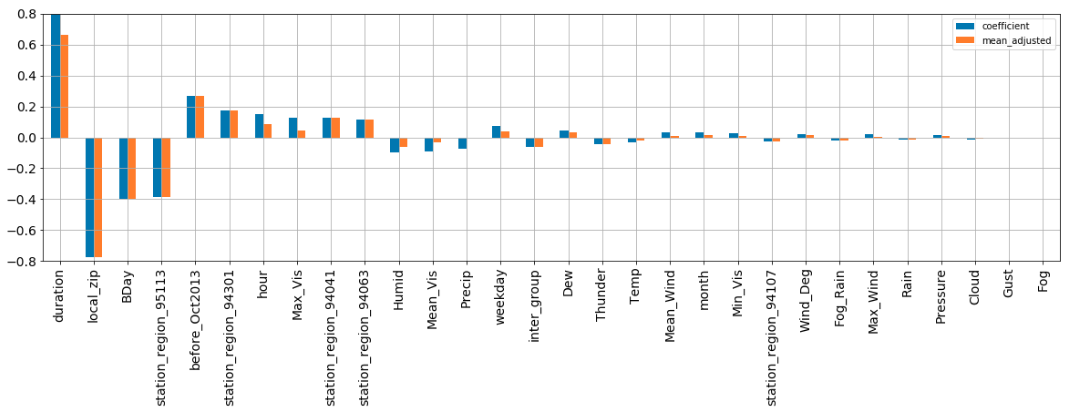
\includegraphics[width=1\textwidth]{FeatureImportanceRidge.png}
					\caption{\label{fig:ridge_importance}The feature importance by RidgeClassifier.}
				\end{subfigure}					
				%
				\begin{subfigure}[b]{1\textwidth}
					\centering
					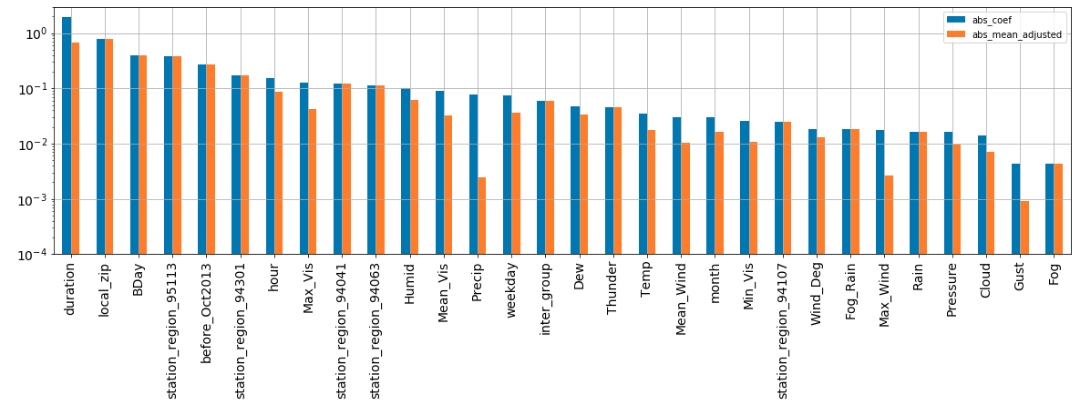
\includegraphics[width=1\textwidth]{ImportanceRidgeAbs.png}
					\caption{\label{fig:ridge_importance_abs}The absolute feature importance by RidgeClassifier.}		
				\end{subfigure}
				\caption{RidgeClassifier importance exploration.}
				\label{fig:ridge_classifier}
			\end{figure}			
			
			The RidgeClassifier, as a linear model, is expected to give very understandable results. Similar with the Lasso model used in the regression problem, adjustment of coefficients for the RidgeClassifier will be applied to make the comparison among feature importance more valid. The result is shown in Figure \ref{fig:ridge_importance}. Also, absolute values of importance are plotted in Figure \ref{fig:ridge_importance_abs}; I set the y axis to be on logarithmic scale to make the feature importance visually more comparable. The patterns of non-subscribers are found as follows:
			
			\begin{itemize}
				\item The duration is the major contributor to the classification. Its positive value suggest that the longer the trip, the more likely the biker is a non-suscriber. Its ranking drops to the second after the adjustment, though.
				
				\item If a biker is from local, it is more likely that he/she is a subscriber as the local\_zip sign is negative. This becomes the most important feature after the adjustment.
				
				\item BDay is negative. More non-subscribers tend to hang out on non-business days.
				
				\item It is quite interesting to see a large negative value for station\_region\_95113, which sort of suggests a share-bike user from San Jose is very unlikely to be a non-subscribers. Does it mean that San Jose is not a very popular city for tourists to come to? Most of San Jose trips are work commuting trips. The station\_region\_94107 is also negative, but with a negligible value. 
				
				On the contrary, the other station groups have relatively large positive values. Does this mean these are tourist-friendly cities? Considering how few trips are in these regions, I'd rather interpret this result as lack of subscribers. People going to work in these regions probably prefer driving than biking.
				
				\item When the bike-sharing program was just launched, people tend to try it out rather than subscribe to the program, which explains the positive sign of the before\_Oct2013 feature.
				
				\item Non-subscribers tend to rent the share-bike at late time in a day for leisure, explaining the positive effect on hour feature.
				
				\item Non-subscribers would prefer to go out when the maximum visibility is high and the mean visibility is low. Non-subscribers are more picky than subscribers on good maximum visibility. The latter is counter-intuitive, but we don't need to worry too much about it. After the adjustment, its value is negligible.
				
				\item Humidity has a negative value. Less non-subscribers would like to go out in more humid days than subscribers do. 
				
				\item The precipitation is also negative, which is expected, because people don't want to hang out when it is raining. However, it becomes a negligible feature after the adjustment. That suggests that non-subscribers are as sensitive to rain as subscribers.
				
				\item The closer to the weekend, the more likely a biker is a non-subscriber: this is understandable for subscribers who use the share-bikes mostly for work commute during working days.
				
				\item Non-subscribers tend not to do inter-group trips. Previous exploration showed that the number of inter-group trips doesn't differ much among subscription groups. This is a sign that feature with importance after this may start becoming irrelevant.
				
				\item The dew point here is the min\_dew\_point. If the minimal dew point is low, it is uncomfortable to people to go out biking. This explains the positive sign.
				
				\item When there is a thunder, non-subscribers are more likely to not rent a bike.
				
				\item The rest are irrelevant features, including temperature, wind speed, month, minimum visibility, San Francisco region, wind degree, fog and / or rain, pressure, cloud, maximum gust speed. It does not mean that these features are not important to non-subscribers, but they have similar influence on all share-bike users.
			\end{itemize}
			
			\subsubsection{Remove the Unimportant Features}
			\paragraph{Remove Unimportant Features Selected by Ridge Classifier.}
			The best way to test whether the unimportant features are truly irrelevant is to remove these features from both the training and testing data and watch the performance change.
			
			Treat all features with absolute adjusted coefficients from the RidgeClassifier smaller than 10\% of the maximum coefficient as irrelevant features. Drop those from the dataset, re-do the fitting and test it on both classifiers. For XGBClassifier, the F0.5 score drops from 0.8519 to 0.8434; for RidgeClassifier, the F0.5 score drops from 0.8073 to 0.8070. The performance does not change significantly. 
			
			Note how many features are left: duration, hour, BDay, local\_zip, before\_Oct2013, station\_region\_94041, station\_region\_94063, station\_region\_94301, station\_region\_95113. Only 9 features are selected out of 30. It is very likely that if the XGBClassifier is re-trained, the result can be better: this will be explored in the next sub-section.
			
			\paragraph{Remove Unimportant Features (by weight) Selected from XGBClassifier.}
			If the same applies to the unimportant features (by weight) selected by the XGBClassifier, the results are much worse. For XGBClassifier, it is 0.7226; for RidgeClassifier, it is 0.6393. Note that 16 features are kept; still the performance is so bad. Again that means the importance ranking by weight is not reliable.
			
			\paragraph{Compare All Importance Rankings.}
			\begin{figure}
				\centering
				\includegraphics[width=1\textwidth]{CompareImportance.png}
				\caption{\label{fig:comp_importance}Compare All XGBClassifier Importance Rankings with that of RidgeClassifier.}	
			\end{figure}
			
			All four importance rankings are plotted on the same figure (Figure \ref{fig:comp_importance}) with the features sorted by the absolute adjusted Ridge coefficients; the Ridge coefficients are normalized before plotting.
			
			The Weight method is clearly out of sync with the Ridge. Same for the Cover method. Blue and green bars still get up high when the red bar diminishes. The Gain method is closest to the Ridge, with only a few discrepancies, e.g. the station\_region\_94107. Since their low importance ends match very well (from Fog\_Rain to Gust), both should be fine when low importance features are of concern. That being said, one still needs to be careful when dealing with the Gain method. Note that the logarithm was applied before normalization to the Gain method. Working on raw importance may lead to erroneous feature selection.

			\subsubsection{Importance Analysis on Dataset with Selected Features}		
			
			\begin{figure}
				\centering
				\includegraphics[width=1\textwidth]{SelImportance.png}
				\caption{\label{fig:sel_importance}Importance comparison on the training set with selected features.}	
			\end{figure}
			
			\begin{figure}
				\centering
				\begin{subfigure}[b]{1\textwidth}
					\centering
					\includegraphics[width=1\textwidth]{SelDurationSplit.png}
					\caption{\label{fig:sel_duration_split}Split points for duration feature.}
				\end{subfigure}					
				%
				\begin{subfigure}[b]{1\textwidth}
					\centering
					\includegraphics[width=1\textwidth]{SelHourSplit.png}
					\caption{\label{fig:sel_hour_split}Split points for hour feature.}		
				\end{subfigure}
				\caption{Split points for numeric features.}
				\label{fig:sel_split}
			\end{figure}		
			
			When the XGBClassifier is tuned on the training set with selected features, the F0.5 score on the testing set goes up a bit from 0.8434 to 0.8447. The importance comparison is shown on Figure \ref{fig:sel_importance}. The result is similar with the previous exploration despite the truncated training set.
			
			There are only two numeric features left, the duration and the hour. If the split points are plotted (Figure \ref{fig:sel_split}), we can see that 10 min is still the most frequently used split point for duration. As for the hour feature, although 12 pm can be a good split point, other values in the afternoon are very close to it, so the split point does not give very helpful information.			
			
			\subsubsection{Explore PCA on the Training Set with Selected Features}
			
			\begin{figure}
				\centering
				\includegraphics[width=1\textwidth]{PCA.png}
				\caption{\label{fig:pca}Principle component analysis.}	
			\end{figure}
			
			Principal component analysis (PCA) is capable of grouping features to manifest important underlying patterns (principal components). To understand more about the data, I apply the PCA to decompose the dataset with unimportant features filtered out according to the suggestion of the Ridge classifier. 
			
			Four components are chosen which together explains over 80\% of the total variance. It is interesting to see how PCA combines different features together to form new features (see Figure \ref{fig:pca}. Supposedly these new features will represent four major patterns of the dataset. NOTE that for each component, only relative signs matter. I will try to interpret the four new features:
			
			The first two new features are mainly the combination of the business day and local zip code in positive correlation and negative correlation. More than half the data variance can be explained by them. Note that both the BDay and the local\_zip features are important for Ridge classifier. 
			
			It is also interesting to see station\_region\_95113 as the third contributing feature. This helps us to understand the PCA components more. 
			
			Since most of the trips don't happen in 94301 (should be in 94107), we can assume the true sign of the station\_region\_95113 is negative as these are the two major components. This means for all regions except the 95113, people can be divided into two groups with distinct pattern of share-bike use: 1) local people using it on business days and 2) local people using it on non-business days. This is reasonable. After all, the majority of share-bike users are subscribers and subscribers are mostly local people.
			
			The third new feature is interestingly a combination of local\_zip and station\_region\_95113. We can somewhat safely assume the positive sign of the station\_region\_95113 to be positive; the third component does not have a great impact on the dataset. People who are local in Bay Area have a very special share-bike activity in San Jose. As explored earlier, we know that this group of people are most likely subscribers.
			
			The fourth new feature emphasizes on the hour and the before\_Oct2013. Before October 2013, people hang out late during the night? This makes sense as there were more non-subscribers when the program just got launched and non-subscribers tend to use the share-bike to enjoy their night life. After October 2013, the pattern reverses.
		
			\subsubsection{Can Deep Learning Improve the Prediction?}			
			
			Deep learning is famous for its performance especially when large amount of data is available. The dataset for the classification problem is somewhat big: it has 30 feature columns and over half a million samples. I would like to apply the deep neural network on the dataset to see if the score can get improved and find out a way to interpret the results. Keras with the tensorflow backend will be used for this study.

			First of all, F0.5 score is not a ready-to-use metric for Keras. A customized F0.5 scoring function is inspired by this \href{https://www.kaggle.com/arsenyinfo/f-beta-score-for-keras}{webpage}. 
			
			A baseline model is created with single fully connected hidden layer with the same number of neurons as input variables. According to this \href{https://machinelearningmastery.com/binary-classification-tutorial-with-the-keras-deep-learning-library/}{link}, this is a good default starting point when creating neural networks.
			
			The baseline model is first tried on the down-sampled dataset, which does not give a promising result at all. The F0.5 score for the testing set is only around 0.5. This is bad even for a baseline model. When the full-sized training set is used, the scores increases to close to 0.8. It indicates that more information will lead to better performance for deep learning models.
			
			The following are tried out to improve the performance of the model:
			
			\begin{itemize}
				\item Optimizers. Learning rate and the decay of the optimizer.
				\item Batch sizes.
				\item Dense and dropout Layers.
				\item Kernal initializer.
				\item Directly work on the full dataset vs first train on the down-sampled.
				\item Activation.
				\item Epochs. 
				\item Class weights.
			\end{itemize}
						
			After all the optimization, the deep learning model with four hidden layers achieves the best score of about 0.84 on the testing set. The training of the model does not always yield the same result, so the best model is saved and loaded for the final prediction. This is a good result, but not very satisfying. It does not do a better job than the XGBClassifier.
			
			\begin{figure}
				\centering
				\includegraphics[width=1\textwidth]{DeepLearningImportance.png}
				\caption{\label{fig:deep_learning}The feature importance of the deep learning model.}	
			\end{figure}
			
			\begin{figure}
				\centering
				\includegraphics[width=1\textwidth]{CompareAll.png}
				\caption{\label{fig:compare_all}The comparison of feature importance ranking among the three classifiers.}	
			\end{figure}
			
			The deep learning model (multilayer perceptron, MLP, here) does not have a built-in function for the feature importance. In fact, the deep learning model is usually depicted as a black box. Nevertheless, I find a general way to test feature importance for any machine learning models. If a feature is important for the model, its value variance must have certain hidden patterns. If these hidden patterns are erased, it must have some impact on the prediction score. The more the impact, the more important the feature. Now that all the data are normalized to have values between 0 and 1, I will set all values of a specific feature column in the testing set to zero and record its F0.5 score. By doing this, the feature importance can be plotted in Figure \ref{fig:deep_learning}. 
			
			The importance can also be calculated as the F0.5 score gain from the least important feature. After normalization, this new importance can be directly compared with the ones with RidgeClassifier and the XGBClassifier (by Gain). Figure \ref{fig:compare_all} shows that the importance calculated this way match that of the other two classifiers for the top four important features. It is more like the XGBClassifier rather than the RidgeClassifier. It marks the hour and the station\_region\_94107 as important features as the XGBClassifiers do, while RidgeClassifier does not agree on that. Although not perfect, this way of calculating the importance does make a lot of sense.
			
			\subsubsection{Discussion on the Difficulties and Complications Encountered During the Implementation}
			
			The classification problem in this project is much more difficult than the regression problem.
			
			First of all, the size of the dataset is much larger. This makes the initial exploration of suitable classifiers extremely difficult, if not impractical at all. So some kind of down sampling is necessary. While there exists tons of discussions on the feature selection on the internet, I could not find any article talking about how to down-size the dataset by truncating the rows instead of the columns. The implemented mechanism in this study by ordering the uniqueness of each feature before compressing the data took me quite some time to figure out. The sample size of 10000 is almost the limit that one can bear with by applying all suitable classifiers on the dataset, otherwise it will take too much time even for the initial classifier filtering.
			
			The xgboost is a very flexible algorithm in parameter tuning to achieve the best performance on a specific dataset. I underestimated the difficulty in manipulating this model. The inner data format it uses is not a pandas dataframe and the F0.5 score has to be defined to be utilized as an evaluation metric for XGBClassifier. The training of the classifier is also different. To have an efficient training process with multiple step grid search, the GPU version of the XGBClassifier is highly recommended. Installing the GPU version was also somewhat challenging; luckily I had already installed the CUDA and CuDNN earlier for a deep learning project, which was a pain. Thanks to the GPU, the XGBClassifier can be trained on the entire dataset to boost the performance to the next level. With CPU, it is just not practical.
			
			The result interpretation is also a challenge as encountered in the regression problem. For XGBClassifier, three feature importances were found. Extra coding was necessary to figure out which one makes more sense. Not surprisingly, a linear model is again required to interpret the result.
			
			One difficulty comes up when I tried to demonstrate a single decision tree out of the XGBClassifier: the default plot setting in xgboost does not allow displaying less depths while the entire tree with nine depths cannot be shown nicely in the notebook or in the project report. In the end, I learned the DOT language that underlies the graphviz and was able to truncate some levels of nodes in the tree to display it in an interpretable way.
			
			The deep learning was explored at the end of the project with the goal of performance boost in expectation. It did not work out as a better model than the XGBClassifier, but the process of exploring this method took quite some time:
			
			\begin{itemize}
				\item The evaluation metric needs customization, which requires the knowledge of the Keras backend functions.
				\item The learning rate was found to be a hidden but rather important parameter for an optimizer.
				\item The batch size was figured out to be causing trouble in testing set evaluation: it could be a bug for the Keras. 
			\end{itemize}   
			
			Lastly, one approach to quantify the feature importance of the deep learning result was invented, which turned out to work well.
			
\clearpage	

	\section{Conclusions and Summary}
	
	\subsection{Conclusions for the Regression Problem}
	The analysis shows that:
	\begin{enumerate}
		\item Cities other than San Francisco are facing a different problem that cannot be directly addressed by machine learning. Only data from San Francisco are suitable for this analysis.
		\item The Gradient Boosting Regressor is a great algorithm in addressing the regression problem among all the available models.
		\item Training datasets with smaller time sections may lead to improvement of the prediction power on a larger time scale dataset.
		\item The time-series treatment of the data is more appropriate, but this dataset shows very limited time dependency. People's behavior on share-bikes does not vary significantly during 2013-2015.
		\item A decision tree based ensemble model captures the feature importance to some extent. Investigating single decision trees in the ensemble could be enlightening. However, its limitation is obvious.
		\item Linear models like the Lasso has a stronger power in terms of result interpretation, even with the sacrifice of the predicting accuracy. 
		\item Removal of irrelevant features picked by the Lasso can improve the performance of the best regressor even if that regressor is not a linear model.
		\item The business day has a major impact on the daily trip counts, with the temperature following it. Both have positive impacts. On events of rain and / or fog, people tend to use the share-bikes less. More docks encourage the bike-sharing in a busy city.
		\item Don't pay attention to the following features: humidity, max and mean visibility, max wind speed, sea level pressure, only fog and the thunder.
		\item Neglecting the irrelevant features, the median prediction error for a particular date in the future is about 81 trips. Comparing to the daily 917 trips in median, this is good enough: the error is less than 10\%. The root mean square logarithmic error is also a good measure of the error.
	\end{enumerate} 
	
	Please refer to Figure \ref{fig:lasso_importance} that shows the feature importance for most of the conclusions drawn above.
	
	\subsection{Conclusions for the Classification Problem}
	To conclude the exploration of the classification problem, there are only a few key features that separate the non-subscribers from subscribers. Please refer to Figure \ref{fig:ridge_classifier} that plots the feature importance for most of the conclusions drawn below.
	
	Non-subscribers tend to have longer trips on non-business days. They are not likely local people. This suggests that a majority of non-subscribers are tourists. It is not practical to convert tourists to subscribers as they do not live in the Bay Area, but the bike-sharing company can consider to offer a weekend pass or holiday pass for these people to encourage them to use the share-bikes.
	
	Non-subscribers are also found to use share-bikes at late time in a day. The company may offer a subscription plan that specifically targets the night users to attract those local people who are not yet subscribers.
	
	It turns out that San Jose is not a popular place for non-subscribers. This may not mean that San Jose is not attractive to tourists. It is possible that the stations are not close to attractions. The company may consider to add stations in points of interest in San Jose.
	
	Other than San Francisco and San Jose, subscribers are relatively rare to find. I suggest the bike-sharing company to collaborate with some companies in Redwood City, Palo Alto and Mountain View to have a program specifically designed for employees. This will improve the usage of share-bikes in these cities.
	
	\subsection{Summary}
	
	This project explores the San Francisco Bay Area bike sharing program by investigating the raw data collected on station, trip, status and weather. I try to answer the following two questions: 
	
	\begin{itemize}
		\item Can we predict the number of trips in a future date?
		\item Can we find some unique patterns for non-subscribers?
	\end{itemize}
		
	The answer to the first question helps the bike-sharing company to  manage the bike re-balancing better. The demand for bikes at smaller time division unit can be explored further based on this study to improve the temporal precision of the prediction.
	
	The answer to the second question helps the bike-sharing company to learn more about their customers, especially those short-term customers. Knowing better about the customers is helpful in finding the pain point they have, addressing which can bring more business to the company.
	
	The raw data are preprocessed to generate proper datasets for these two questions. Appropriate machine learning models are then applied and optimized to obtain good scores upon carefully selected metrics.
	
	One thing to clarify for finding the best model. I don't check a statistical test in my study.  \href{http://www.site.uottawa.ca/ICML08WS/papers/J_Demsar.pdf}{One paper} suggests that it is in general not applicable for machine learning. I don't have the expertise to judge whether this is true as I don't come from the statistics background. Nevertheless, considering that the amount of samples is much larger than the typical threshold of 30 and the distribution of the samples is not normal, it is neither necessary nor proper to apply the t-test to verify whether the chosen model works better than the benchmark model. More specifically to the classification problem, due to the imbalanced data, the accuracy is not an adequate metric while it is the underlying measure for a general statistical significance test, which invalidates the statistical tests. 
	
	Obtaining the best-performing model is one thing, the other critical matter is the interpretability. While predicting the result is important, understanding it is as important. The power of any data analysis is to assist the decision making. Machine learning, as a type of data analysis, is no difference. Good prediction helps to see the future; good understanding of the problem helps to shape the future.
		
	This project will end here, but this is not the end for problem solving. 
	
	First of all, this project is not meant for an exhaustive analysis on all aspects of the data. There are still unexplored questions. For example, will even smaller time sections improve the prediction further? Will the number of available bikes in a station affects the decision of a non-subscriber? What about how old the bike is? 
	
	Secondly, the data itself is not completely self-consistent as extra trips are found in the status data in comparison to the trip data. The missing information prevents certain data analysis. 
	
	Lastly, the data analysis is only part of the problem solving process, it is simply paving the road for the solution to real-world problems. This analysis needs to be integrated into the everyday business operation to leverage its power. Also, keep in mind that the world is changing, so the analysis needs to be updated accordingly.
			
\clearpage										
		
	\begin{appendix}
		\listoffigures
	\end{appendix}
	
\end{document}